%%%%%%%%%%%%%%%%%%%%%%%%%%%%%%%%%%%%%%%%%%%%%%%%%%%%%%%%%%%%%%%%%%%%%%
% Universidade Federal de Santa Catarina
% Biblioteca Universitária
%
% (c)2010 Roberto Simoni (roberto.emc@gmail.com)
%         Carlos R Rocha (cticarlo@gmail.com)
%%%%%%%%%%%%%%%%%%%%%%%%%%%%%%%%%%%%%%%%%%%%%%%%%%%%%%%%%%%%%%%%%%%%%%%
%\PassOptionsToPackage{abnt-etal-cite=1, abnt-etal-list=0}{abntcite}
\documentclass{ufscThesis}

%%%%%%%%%%%%%%%%%%%%%%%%%%%%%%%%%%%%%%%%%%%%%%%%%%%%%%%%%%%%%%%%%%%%%%%
% Pacotes usados especificamente para este documento
% Definidos pelo criador do documento
%%%%%%%%%%%%%%%%%%%%%%%%%%%%%%%%%%%%%%%%%%%%%%%%%%%%%%%%%%%%%%%%%%%%%%%
\usepackage{booktabs}
\usepackage{multirow}
\usepackage{graphicx}
\usepackage[ruled]{algorithm2e}
\usepackage[table,xcdraw]{xcolor}
\usepackage{lipsum}
\usepackage{amsmath}
\usepackage{amsfonts}
\usepackage{url}
\usepackage{rotating}
\usepackage{float}
\usepackage{pdfpages}
%%%%%%%%%%%%%%%%%%%%%%%%%%%%%%%%%%%%%%%%%%%%%%%%%%%%%%%%%%%%%%%%%%%%%%%
% Pacotes usados especificamente para este documento
% Definidos pelo AUTOR
%%%%%%%%%%%%%%%%%%%%%%%%%%%%%%%%%%%%%%%%%%%%%%%%%%%%%%%%%%%%%%%%%%%%%%%
\usepackage[printonlyused, withpage]{acronym}
\usepackage{subfigure}
\usepackage{booktabs}
\usepackage{lscape}
%%%%%%%%%%%%%%%%%%%%%%%%%%%%%%%%%%%%%%%%%%%%%%%%%%%%%%%%%%%%%%%%%%%%%%%
% Comandos usados especificamente para este documento
% Definidos pelo AUTOR
%%%%%%%%%%%%%%%%%%%%%%%%%%%%%%%%%%%%%%%%%%%%%%%%%%%%%%%%%%%%%%%%%%%%%%%
\newcommand\todo[1]{\textcolor{red}{TODO: #1}}

%%%%%%%%%%%%%%%%%%%%%%%%%%%%%%%%%%%%%%%%%%%%%%%%%%%%%%%%%%%%%%%%%%%%%%%

%\renewcommand{\theequation}{\arabic{equation}} %se desejar tirar o capitulo

%\usepackage[labelsep=period]{caption} % O separador de legenda é um .
\usepackage[labelsep=endash]{caption} % O separador de legenda é um -

%%%%%%%%%%%%%%%%%%%%%%%%%%%%%%%%%%%%%%%%%%%%%%%%%%%%%%%%%%%%%%%%%%%%%%%
% Identificadores do trabalho
% Usados para preencher os elementos pré-textuais
%%%%%%%%%%%%%%%%%%%%%%%%%%%%%%%%%%%%%%%%%%%%%%%%%%%%%%%%%%%%%%%%%%%%%%%
\titulo{Avaliação quantitativa do impacto da organização dos dados no contexto de Physical Design}
%\subtitulo{Estilo \LaTeX~ padrăo}                % Subtitulo do trabalho (opcional)
\autor{Tiago Augusto Fontana}                     % Nome do autor
\data{}{Novembro}{2017}                           % Data da publicaçăo do trabalho

\orientador{Prof.\ Dr.\ José\ Luís\ Almada\ Güntzel} % Nome do orientador e (opcional) seu título
%\coorientador{Prof. Dr. Beltrano}                % Nome do coorientador e seu título (opcional)
%\coordenador{Prof. Chefe, Dr. Eng.}              % Nome do coordenador do curso e (opcional) seu título

\departamento{Programa de Pós-Graduação em Ciência da Computação}
\curso{Programa de Pós-Graduação em Ciência da Computação}

\documento[a]{Dissertação}
\grau{Mestre em Ciência da Computação}


%%% Sobre a Banca
\numerodemembrosnabanca{3} % Isso decide se haverá uma folha adicional
\orientadornabanca{sim} % Se faz parte da banca definir como sim
%\coorientadornabanca{sim} % Se faz parte da banca definir como sim
\bancaMembroA{Dr.\ José\ Luis\ Almada\ Güntzel} %Nome do presidente da banca
\bancaMembroB{Dr.\ }      % Nome do membro da Banca
\bancaMembroC{Dr.\ }       % Nome do membro da Banca
% \bancaMembroD{Dr.\ }     % Nome do membro da Banca
%\bancaMembroE{Prof. quinto membro}       % Nome do membro da Banca
%\bancaMembroF{Prof. sexto membro}        % Nome do membro da Banca
%\bancaMembroG{Prof. sétimo membro}       % Nome do membro da Banca

\dedicatoria{A quem o trabalho é dedicado, se é que o é (opcional)}

\agradecimento{Agradeço ao meu orientador José Luís Almada Güntzel, por todo o auxílio oferecido
na execução deste trabalho e na escrita deste texto. \\
Agradeço aos membros da banca, por cederem seu tempo para a avaliação deste trabalho. \\
% Agradeço aos meus colegas de trabalho Vinicius dos Santos Livramento e Chrystian de Sousa Guth,
% pela ajuda durante a realização deste trabalho. \\
% Agradeço à minha namorada Taciane Martimiano, por me acompanhar nestes dois anos de mestrado. \\
% Por fim, agradeço à minha família Carlos Alberto Barbosa Netto, Loreni Oliveira Netto e Caio Oliveira Netto,
% por todo apoio e dedicação oferecidos até hoje, pois sem eles, nada disso seria possível.
}

\epigrafe{Um bonito pensamento ou citaçăo, se for o caso}{autor do pensamento}

% \textoResumo{ }

% \palavrasChave{ }

% \textAbstract{ }

% \keywords{ }

%%%%%%%%%%%%%%%%%%%%%%%%%%%%%%%%%%%%%%%%%%%%%%%%%%%%%%%%%%%%%%%%%%%%%%%
% Início do documento
%%%%%%%%%%%%%%%%%%%%%%%%%%%%%%%%%%%%%%%%%%%%%%%%%%%%%%%%%%%%%%%%%%%%%%%
\begin{document}

%--------------------------------------------------------
% Elementos pré-textuais
\capa
%\folhaderosto[comficha] % Se nao quiser imprimir a ficha, é só năo usar o parâmetro
\folhaderosto% Se nao quiser imprimir a ficha, é só năo usar o parâmetro
% \includepdf[pages={1}]{capitulos/ficha_catalografica.pdf}
% 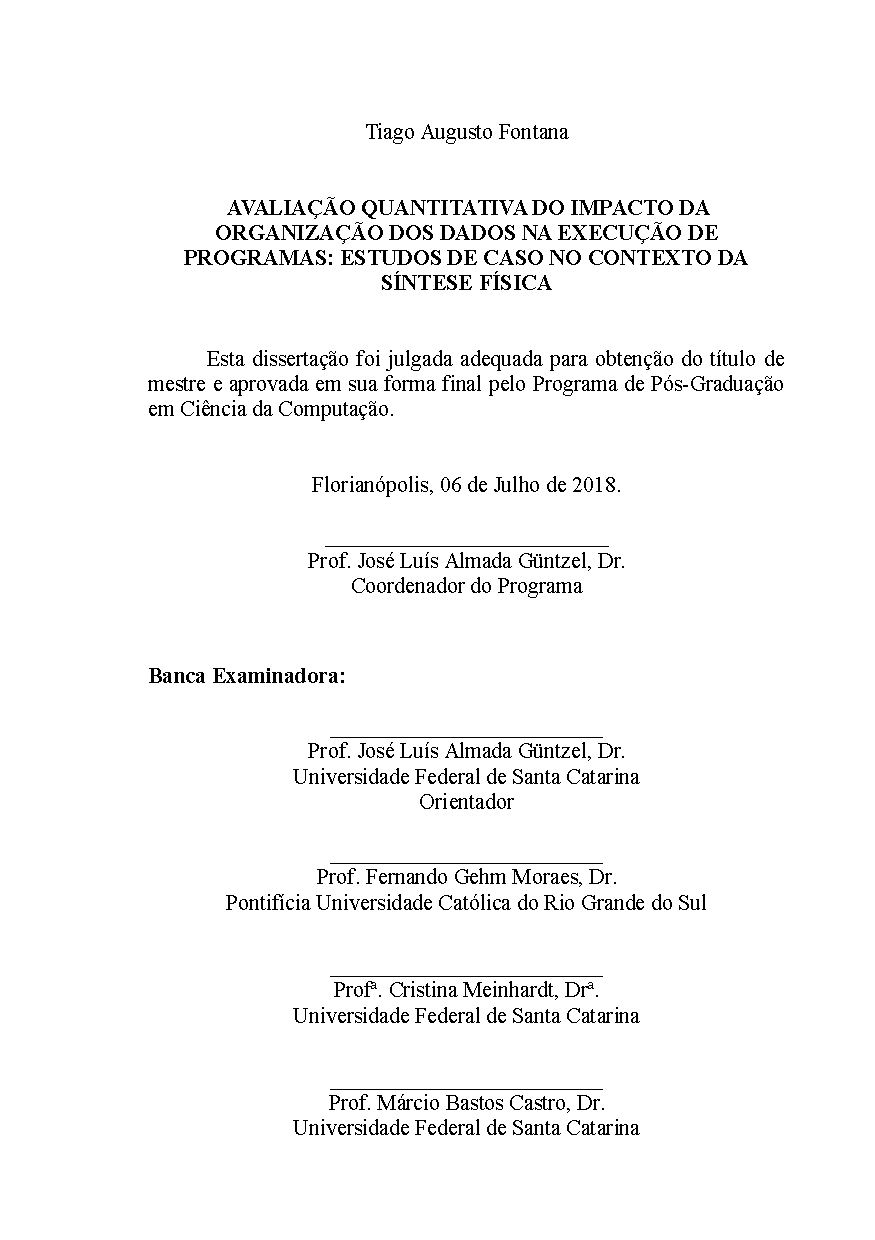
\includepdf{capitulos/aprovacao.pdf}
%\paginadedicatoria
%\paginaagradecimento
%\paginaepigrafe
\textoResumo{ 

As ferramentas de Physical Design devem lidar com uma grande quantidades de dados para resolver problemas de circuitos com milhões de células.
Tradicionalmente, as ferramentas de \textit{Eletronic Design Automation} (EDA) são implementadas usando o paradigma de programação orientado a objetos (OOD).
No entanto, usar esse paradigma pode levar a objetos excessivamente complexos que resultam em desperdício de espaço de memória.
Esse desperdício de memória prejudica a exploração da localidade da memória cache e, consequentemente, degrada o tempo de execução do software.
Este trabalho propõe uma organização eficiente dos dados para três algoritmos diferentes de \textit{Physical Design}.
Para esta organização de dados, este trabalho aplica o modelo orientado a dados \textit{Data-Oriented Design}(DOD).
Diferentemente do modelo tradicional orientado a objetos, o modelo de programação de orientado a dados se concentra em como os dados são organizados na memória.
Como consequência, este modelo de programação pode explorar melhor a localidade espacial da cache e reduzir o tempo total de execução.
Para avaliar o impacto do uso do modelo de programação Data-Oriented Design, implementamos dois protótipos de software (uma implementação sequencial e uma paralela) de algoritmos de \textit{Physical Design} para cada um dos modelo de programação.
Os resultados experimentais preliminares mostraram que a implementação do orientada a dados (Data-Oriented Design) reduz o número total de \textit{cache misses} e é mais rápido do que a implementação com o paradigma Orientado a Objetos.

}
\palavrasChave{ 
Localidade da Cache; Eletronic Design Automation; Physical Design; Otimização de Software; Data-Oriented Design.
}

\textAbstract{ 

Physical design tools must handle huge amounts of data in order to solve problems for circuits with millions of cells. 
Traditionally, Electronic Design Automation (EDA) tools are implemented using Object-Oriented Design (OOD).
However, using this paradigm may lead to overly complex objects that result in waste of cache memory space.
This memory wasting harms cache locality exploration and, consequently, degrades software runtime. 
This work proposes an efficient organization of the data for three different algorithms of Physical Design.
For this data organizatio, this work apply Data-Oriented Design.
Differently from the traditional Object-Oriented design, the Data-Oriented Design programming model focus on how the data is organized in the memory.
As consequence, this programming model may better explore cache spatial locality and reduce the total runtime.
In order to evaluate the impact of using the Data-Oriented Design programming model, we implemented two software prototypes (a sequential and a parallel implementation) of Physical Design algorithms for each programming model.
Preliminary experimental results showed that the Data-Oriented Design implementation reduces the total number of cache misses and it is more faster than Object-Oriented Design implementation.

}
\keywords{ 
Cache Locality; Eletronic Design Automation; Physical Design; Software Optimization; Data-Oriented Design.
}
\paginaresumo
\paginaabstract
\listadefiguras
\listadetabelas
\begin{singlespacing}
\chapter * {Lista de Abreviaturas e Siglas}
\thispagestyle{empty}
\label{acro}
%\addcontentsline{toc}{chapter}{Lista de Acr�nimos}
%\begin{tabbing}

%\singlespace

\begin{acronym}
\setlength{\parskip}{0ex}
\setlength{\itemsep}{1ex}

%\begin{singlespace}

\renewcommand{\baselinestretch}{0.25}%
\large\normalsize%



% +++++ TIAGO +++++
% A

% B

% C

% D
\acro{dme}[DME]{\textit{Deferred-Merge Embedding}}
\acro{dod}[DOD]{Data-Oriented Design}

% E
\acro{ecl}[ECL]{Laboratório de ComputaçãSo Embarcada - \textit{Embedded Computing Lab}}
\acro{eda}[EDA]{Electronic Design Automation}

% F

% G

% H

% I
\acro{ic}[IC]{Circuito Integrado - \textit{Integrated Circuit}}
\acrodefplural{ic}[ICs]{Circuitos Integrados - \textit{Integrated Circuits}}

% J

% L

% M
\acro{mmm}[MMM]{Método de Médias e Medianas - \textit{Method of Means and Medians}}

% N

% O
\acro{ood}[OOD]{Object-Oriented Design}

% P

% Q

% R
\acro{rgm}[RGM]{Adequação Geométrica Recursiva - \textit{Recursive Geometric Matching}}

% S

% T

% U

% V
\acro{vlsi}[VLSI]{\textit{Very-large-scale Integrated}}




% andre
\acro{3ccd}[3 CCD]{\textit{Three-CCD}}
\acro{a1csa}[A1CSA]{\textit{Add-One Carry-Select Adder}}
\acro{a1csah}[A1CSAH]{\textit{Hierarchical Add-One Carry-Select Adder}}
\acro{ads}[ADS]{\textit{Absolute Difference of Sums}}
\acro{anova}[ANOVA]{Análise de Variância - \textit{Analysis of Variance}}
\acro{aps}[APS]{\textit{Alternating pel-subsampling block matching algorithm}}
\acro{asic}[ASIC]{\textit{Application Specific Integrated Circuit}}
\acro{AVCHD}{\textit{Advanced Video Codec High Definition}}
\acro{b}[B]{Bipredito}
\acro{bdbr}[BDBR]{\textit{Bjontegaard Delta Bitrate}}
\acro{bdpsnr}[BDPSNR]{\textit{Bjontegaard Delta PSNR}}
\acro{bm}[BM]{\textit{Block Matching}}
\acro{ccd}[CCD]{Dispositivo de Carga-Acoplada - \textit{Charge-Coupled Device}}
\acro{cla}[CLA]{\textit{Carry-Lookahead Adder}}
\acro{cmos}[CMOS]{Semicondutor Metal-Óxido Complementar - \textit{Complementary Metal-Oxide Semiconductor}}
\acro{cra}[CRA]{\textit{Carry-Ripple Adder}}
\acro{csa}[CSA]{\textit{Carry-Select Adder}}
\acro{dag}[DAG]{Grafo Acíclico Direcionado - \textit{Direct Acyclic Graph}}
\acro{dc}[DC]{\textit{Direct Current}}
\acro{sdc}[DC]{\textit{Synopsys Design Compiler}}
\acro{dct}[DCT]{Transformada Discreta dos Cossenos - \textit{Discrete Cosine Transform}}
\acro{dpcm}[DPCM]{Modulação por Codificação de Pulso Diferencial - \textit{Differential pulse-code modulation}}
\acro{ds}[DS]{\textit{Diamond Search}}
\acro{dsp}[DSP]{\textit{Digital Signal Processing}}
\acro{dssim}[DSSIM]{Índice de Dissimilaridade Estrutural - \textit{Structural Dissimilarity Index}}
\acro{dst}[DST]{Transformada Discreta dos Senos - \textit{Discrete Sine Transform}}
\acro{DVD}{Disco de Vídeo Digital - \textit{Digital Video Disc -}}
\acro{esa}[ESA]{Algoritmo de Busca por Eliminações Sucessivas - \textit {Successive Elimination Exhaustive Search Algorithm}}
\acro{fbma}[FBMA]{\textit{Fullsearch Block Matching Algorithm}}
\acro{fbsme}[FBSME]{Estimação de Movimento para Blocos de Tamanho Fixo - \textit{Fixed Block-Size Motion Estimation}}
\acro{fft}[FFT]{Transformada Rápida de Fourier - \textit{Fast Fourier Transform}}
\acro{fme}[FME]{\textit{Fractional Motion Estimation}}
\acro{fpga}[FPGA]{\textit{Field-Programmable Gate Array}}
\acro{fps}{Quadros por Segundo - \textit{Frames per Second}}
\acro{fr}[FR]{Taxa de Quadros - \textit{Frame Rate}}
\acro{fssd}[FSSD]{Soma das Diferenças Quadráticas Rápida - \textit{Fast Sum of Squared Differences}}
\acro{fsm}[FSM]{Máquina de Estados Finitos - \textit{Finite State Machine}}
\acro{ga}[GA]{Algoritmo Genético - \textit{Genetic Algorithm}}
\acro{gcc}[GCC]{\textit{GNU Compiler Collection}}
\acro{gea}[GEA]{Algoritmo de Eliminação Global - \textit{Global Elimination Algorithm}}
\acro{gnu}[GNU]{``\textit{GNU's Not Unix}!''}
\acro{gpl}[GPL]{\textit{General Public License}}
\acro{HD-DVD}{\textit{High Definition Digital Video Disc}}
\acro{HD}{Alta Definição - \textit{High Definition}}
\acro{hevc}[HEVC]{Codificação de Vídeo de Alta Eficiência - \textit{High Efficiency Video Coding}}
\acro{hw}[HW]{Hardware}
\acro{hvs}[HVS]{Sistema Visual Humano - \textit{Human Visual System}}
\acro{i}[I]{Intra}
\acro{ifa}[IFA]{\textit{Internationale Funkausstellung Berlin}}
\acro{irs}[IRS]{Busca Aleatória Iterativa - \textit{Iterative Random Search}}
\acro{itut}[ITU-T]{\textit{International Telecommunication Union Telecommunication Standardization Sector}}
\acro{jm}[JM]{\textit{Joint Model}}
\acro{jvt}[JVT]{\textit{Joint  Video Team}}
\acro{lh}[LH]{\textit{Low-Vdd/High-Vt}}
\acro{mad}[MAD]{\textit{Mean Absolute Difference}}
\acro{mb}[MB]{Macrobloco - \textit{Macroblock}}
\acro{mc}[MC]{Compensação de Movimento - \textit{Motion Compensation}}
\acro{me}[ME]{Estimação de Movimento - \textit{Motion Estimation}}
\acro{MPEG-2}{\textit{Moving Pictures Expert Group} - 2}
\acro{mpeg}[MPEG]{\textit{Moving Picture Experts Group}}
\acro{mse}[MSE]{\textit{Mean Squared Error}}
\acro{mv}[MV]{Vetor de Movimento - \textit{Motion Vector}}
\acro{nn}[NN]{Nominal}
\acro{NTSC}{\textit{National Television System Committee}}
\acro{p}[P]{Predito}
\acro{p2p}[P2P]{Ponto-a-Ponto - \textit{Peer-to-Peer}}
\acro{pdp}[PDP]{Produto Atraso-Potência - \textit{Power-Delay Product}}
\acro{pmd}[PMD]{Dispositivo Móvel Portátil - \textit{Portable Mobile Device}}
\acro{pmv}[PMV]{Vetor de Movimento Predito - \textit{Predicted Motion Vector}}
\acro{psnr}[PSNR]{Relação Sinal-Ruído de Pico - \textit{Peak signal-to-noise ratio}}
\acro{QDE}{\textit{Quantized Distortion Energy}}
\acro{qme}[QME]{\textit{Quartet-pel motion estimation}}
\acro{qsds-dic}[QSDS-DIC]{\textit{Quarter Sub-sampled Diamond Search algorithm with Dynamic Iteration Control}}
\acro{rbsad}[RBSAD]{\textit{Reduced Bit Sum of Absolute Differences}}
\acro{rd}[RD]{Taxa-Distorção - \textit{Rate-Distortion}}
\acro{rdo}[RDO]{Otimização Taxa-Distorção - \textit{Rate-Distortion Optimization}}
\acro{rgb}[RGB]{Vermelho, Verde e Azul - \textit{Red, Green and Blue}}
\acro{saif}[SAIF]{\textit{Switching Activity Interchange Format}}
\acro{sad}[SAD]{Soma das Diferenças Absolutas - \textit{Sum of Absolute Differences}}
\acro{satd}[SATD]{Soma das Diferenças Transformadas Absolutas - \textit{Sum of Absolute Transformed Differences}}
\acro{SBTVD}{Sistema Brasileiro de Televisão Digital}
\acro{sea}[SEA]{Algoritmo de Eliminações Sucessivas - \textit{Sucessive Elimination Algorithm}}
\acro{SL}{Camada Simples - \textit{Single Layer}}
\acro{ssd}[SSD]{Soma das Diferenças Quadráticas - \textit{Sum of Squared Differences}}
\acro{ssim}[SSIM]{Índice de Similaridade Estrutural - \textit{Structural Similarity Index}}
\acro{tsmc}[TSMC]{\textit{Taiwan Semiconductor Manufacturing Company Limited}}
\acro{tss}[TSS]{\textit{Three-Step Search}}
\acro{tu}[TU]{\textit{Transform Unit}}
\acro{v1}[V1]{Córtex Visual Primário}
\acro{v2}[V2]{Área visual V2}
\acro{vcs}[VCS]{\textit{Synopsys VCS}}
\acro{vecg}[VECG]{\textit{Visual Coding Experts Group}}
\acro{vbs}[VBS]{Tamanho de Bloco Variável - \textit{Variable Block Size}}
\acro{vbsme}[VBSME]{Estimação de Movimento para Blocos de Tamanho Variável - \textit{Variable Block Size Motion Estimation}}

\acro{vod}[VoD]{Vídeo sob Demanda - \textit{Video on Demand}}
\acro{vpi}[VPI]{\textit{Verilog Procedural Interface}}
\acro{ycbcr}[Y'CbCr]{Y' (luma) Cb e Cr (\textit{``blue-difference''} e \textit{``red-difference''}) dos componentes de cor}


\renewcommand{\baselinestretch}{1}%
\large\normalsize%

%\end{singlespace}
\end{acronym}
%\end{tabbing}
\end{singlespacing}
% \listadeabreviaturas
\listadesimbolos
\sumario

%-------------------------------------------------------------------------------
% Para listagens de algoritmos e de código, recomenda-se consultar os
% pacotes algorithms e lstlistings, que săo usados para definir esses
% dois tipos de elementos de texto e possuem os comandos
% \listofalgorithms e \lstlistoflistings, respectivamente.
%-------------------------------------------------------------------------------

%--------------------------------------------------------
% Elementos textuais



\chapter{Introdução}
\label{cap:introducao}
    % evolução da tecnologia -> transistores menores
    % circuitos modernos muito grande grandes -> ferramentas de EDA
    % eletrônica de consumo -> tempo limitado para projeto de um circuito
    % é benéfico a redução de tempo na execução dos algoritmos sem perda da qualidade da solução
    % memória representa gargalo -> explorar a localidade na cache
    %
    % uma possível solução que não altera a qualidade da solução é o melhor armazenamento dos dados

A evolução da tecnologia de fabricação de \acp{ic} vem permitindo uma redução drástica e contínua das dimensões dos transistores.
O consequente aumento de densidade permite a fabricação de \acp{ic} com um número cada vez maior de transistores, podendo chegar a milhões de transistores.
Além disso, os circuitos contemporâneos devem respeitar uma ampla gama de restrições, sejam elas de atraso, potência e\@/\@ou área.
Adicionalmente, o processo de projeto e fabricação possui um tempo limitado para que um novo eletronico possa garantir o mercado.
Portanto, as Ferramentas de \ac{eda} são obrigatórias no design de \acp{ic} modernos.




ferramentas seguem um fluxo de projeto
explicar o fluxo
varias etapas do fluxo podem voltar
dados das etapas podem ser reutilizados
é benefico uma melhor organização dos dados


Essas ferramentas de \ac{eda} devem tratar um grande volume de dados em um curto período de tempo. Portanto, essas ferramentas de \ac{eda} devem empregar otimizações de software, como o uso de melhores estruturas de dados, paralelização e exploração de local de cache.

modelagem dos dados deve ser ótima para diversas relações
OOD pode gerar uma hierarquia muito complexa e problemas sem solução (a não ser replicação do código)








este trabalho avalia o impacto da exploração da localidade do cache no agrupamento de registros.


\section{Justificativa}
    o que a literatura não fez
    Portanto, é desejável o desenvolvimento ... sobretudo uma comparação que faça uso de uma infraestrutura realista.

\section{Objetivos e Contribuições Pretendidas}
        Objetivo
            Este trabalho tem como objetivo a avaliação quantitativa do impacto de diferentes
        Objetivos específicos

        Contribuições científicas e tecnológicas
            avaliação quantitativamente do desempenho causado pela modelagem dos dados em três tarefas da síntese física
            Resultados experimentais utilizando uma infraestrutura baseada em circuitos industriais,

\section{Metodologia}
        Implementar versões de problemas
        avaliar quantitativamente o número de cache misses
        avaliar quantitativamente o tempo de execução

\section{Limitações(escopo) deste trabalho}
        somente 3 problemas avaliados
        somente uma arquitetura de processador e cache
        paralelização com um chunk único

\section{Organização deste trabalho}

    % contextualização     do     problema;
    % objetivos;
    % metodologia;
    % contribuições;
\chapter{Trabalhos correlatos}
\label{cap:trabalhos_correlatos}

% Este capítulo apresenta os principais trabalhos correlatos no contexto do problema de legalização. Inicialmente, são revisados os principais algoritmos de legalização completa. Em seguida, são descritos os principais algoritmos propostos para resolver o problema de legalização incremental. É importante ressaltar que este capítulo não faz uma análise exaustiva dos algoritmos de legalização, mas busca apresentar os trabalhos mais relevantes relacionados às diferentes abordagens utilizadas para resolver o problema.

% \section{Trabalhos correlatos em legalização completa}

    % revisão bibliográfica;
% !TEX root = ../dissertacao.tex
\acresetall{}
\chapter{Explorando a localidade dos dados em Physical Design Automation}
\label{cap:tecnica_proposta}

Este capítulo apresenta a proposta de organização dos dados para melhorar o desempenho de tarefas de Physical Design Automation.
Inicialmente será revisado alguns conceitos básicos de acesso a memoria principal para recuperação dos dados.
Em seguida, serão discutidas as limitações do modelo \ac{ood} e como o modelo Orientado a Dados (DOD) pode sanar os mesmos.
% Por fim, será apresentado como aplicar os dois modelos (OOD e DOD) em três tarefas de Physical Design.
Por fim, na Seção~\ref{sec:entity_component_system}, será apresentado um padrão de projeto para facilitar o acesso as dados organizados segundo modelo \ac{dod}.

A arquitetura de memória de computadores modernos é tipicamente hierárquica como mostrado na Figura~\ref{fig:memoryHierarchy}. Observe que os níveis mais baixos na hierarquia (por exemplo, disco rígido e memória principal) têm maior capacidade, mas possuem maior latência. Por outro lado, os níveis mais altos (por exemplo, memória cache e registradores da CPU) são rápidos, mas possuem capacidade limitada. Quando um determinado programa precisa um dado, e o mesmo não se encontra nos registradores da CPU, será realizado uma busca por este dado nos níveis mais altos da hierarquia da  cache. Quando os dados não são encontrados em algum dos níveis de cache, dizemos que ocorreu um \textbf{cache miss}. Quando um cache miss ocorre, os dados são acessados no nível inferior da hierarquia. No pior caso, este dado será recuperado do disco rígido e levado por todos os níveis da hierarquia. Quando o dado buscado é recuperado para a cache de mais alto nível e posteriormente armazenado num registrador da CPU, o programa que estava acessando os dados volta a executar. Caso que esses dados forem necessários novamente, e o bloco da cache não tenha sido sobrescrito, eles estarão disponível na cache e sua busca nos níveis da cache resultará em \textbf{cache hit}~\cite{patterson2013computer}.

\begin{figure}[ht]
    \centering
    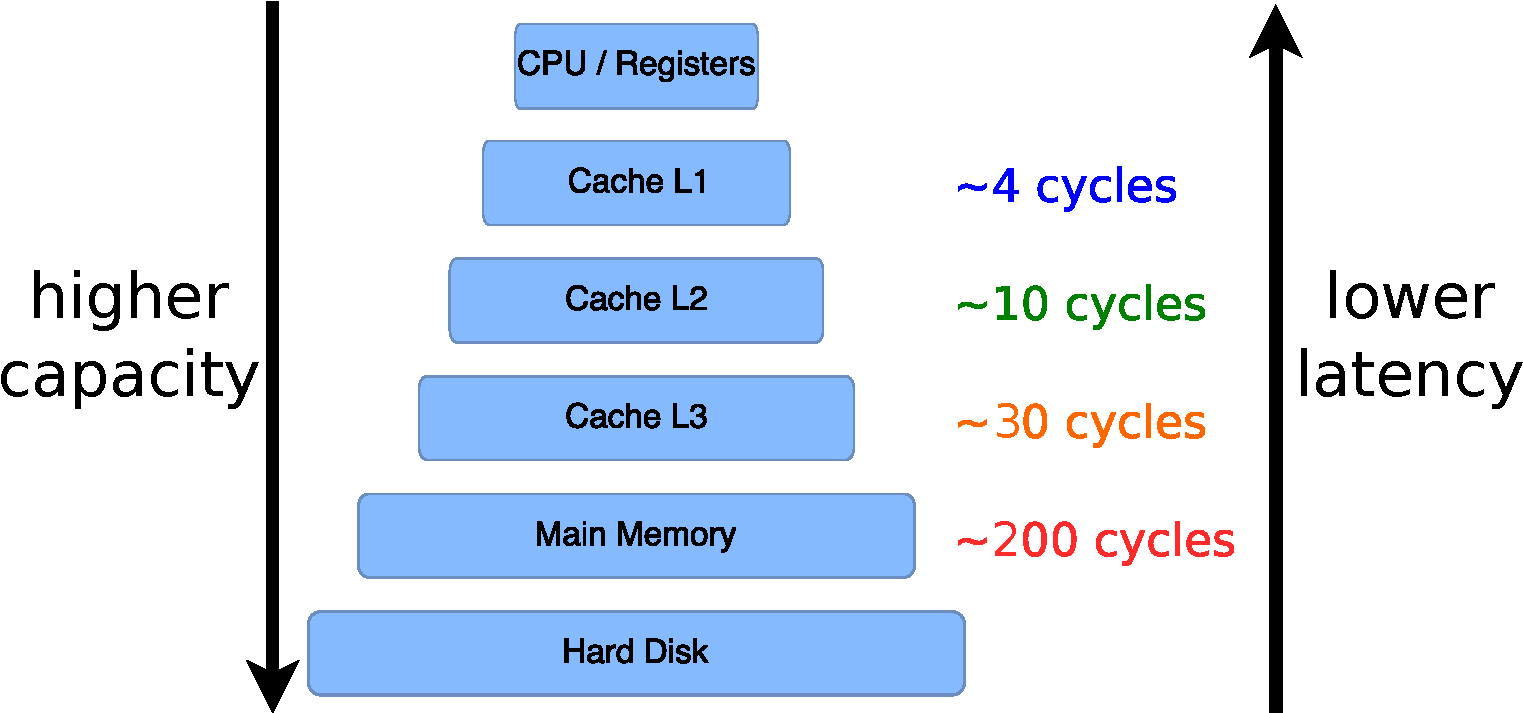
\includegraphics[width=0.7\linewidth]{img/tecnica/memoryHierarchy}
    % \caption{Hierarchy of memory present in modern computers. The hierarchy is compose by hard disk, main memory, three levels of cache and CPU registers. Adapted from~\cite{patterson2013computer}.}
    \caption[Hierarquia de memória]{Hierarquia de memória presente em computadores modernos. A hierarquia é composta por disco rígido, memória principal, três níveis de cache e registradores. Adaptada de~\cite{patterson2013computer}.}
    \label{fig:memoryHierarchy}
\end{figure}

A localidade espacial da cache (\textit{cache spatial locality}) é uma propriedade importante dos sistemas hierárquicos de memória. Esta propriedade afirma que a probabilidade de acessar um recurso da memória é maior se um recurso próximo já foi referenciado~\cite{patterson2013computer}. O sistema de cache explora esta propriedade armazenando os dados em blocos (\textit{cache blocks}). Sempre que algum dado é acessado a partir da memória principal, ele é recuperado para a cache juntamente com outros dados que estavam armazenados próximos a ele. Desta forma, se os dados próximos forem acessados posteriormente, resultarão em cache hits.

É possível explorar ainda mais a localidade espacial do cache, mudando a forma como os dados são organizados em um determinado software mesmo não possuindo nenhuma informação de qual será a organização e tamanho da cache.
Isto é possível uma vez que ao armazenar dados de uma mesma categoria de forma contígua estamos aumentando a probabilidade de um acesso gerar um cache hit.

Por exemplo, um algoritmo de Clusterização de Registradores executa operações em todas as posições dos registradores de um circuito.
Ao armazenar todas as posições dos registradores em um único vetor contíguo, este algoritmo irá necessitar de um número inferior de cache misses para recuperar todos os dados.
Como consequência, o tempo de acesso a dados é reduzido e o desempenho do software é melhorado. Esta organização de dados nem sempre é eficientemente feita pelo modelo de programação tradicional~\ac{ood}.
Neste modelo de programação, os dados são armazenados agrupando todas as informações de um mesmo objeto num único registro.
Observe que com esta abordagem, quando os objetos são recuperados para a cache, alguns dados inúteis (atributos do objeto) são carregados juntos. Portanto, a cache é desperdiçado com dados que provavelmente não serão utilizados pelo algoritmo.

Uma alternativa para o modelo de \ac{ood} é o modelo de programação \ac{dod}. Este modelo tem como enfoque a forma como os dados são organizados na memória.
% A Figura~\ref{fig:entityPropertyDOD} mostra um exemplo sobre como modelar os dados usando este modelo de programação.
Enquanto no modelo \ac{ood} utiliza objetos complexos e seus atributos para representar os objetos do mundo real, o modelo \ac{dod} representa os dados do mundo real como entidades e suas propriedades (atributos).
Cada entidade é simplesmente um índice. Este índice é utilizado para acessar suas propriedades.
Assim, cada propriedade pode ser armazenada num único vetor contíguo na memória.
% Por exemplo, na Figura~\ref{fig:entityPropertyDOD}, o vetor de entidades armazenam todos os índices das entidade, enquanto os outros vetores armazenam suas propriedades, as quais podem ser acessadas usando os índices do vetor de entidades.
Ao organizar os dados dessa forma, quando um algoritmo precisa apenas de uma propriedade (por exemplo a posição dos registradores) ele pode recuperar somente o vetor que contem estes dados.
Desta forma, não são recuperados dados desnecessários o que acarreta numa maior localidade espacial da cache.

% \begin{figure}[ht]
%     \centering
%     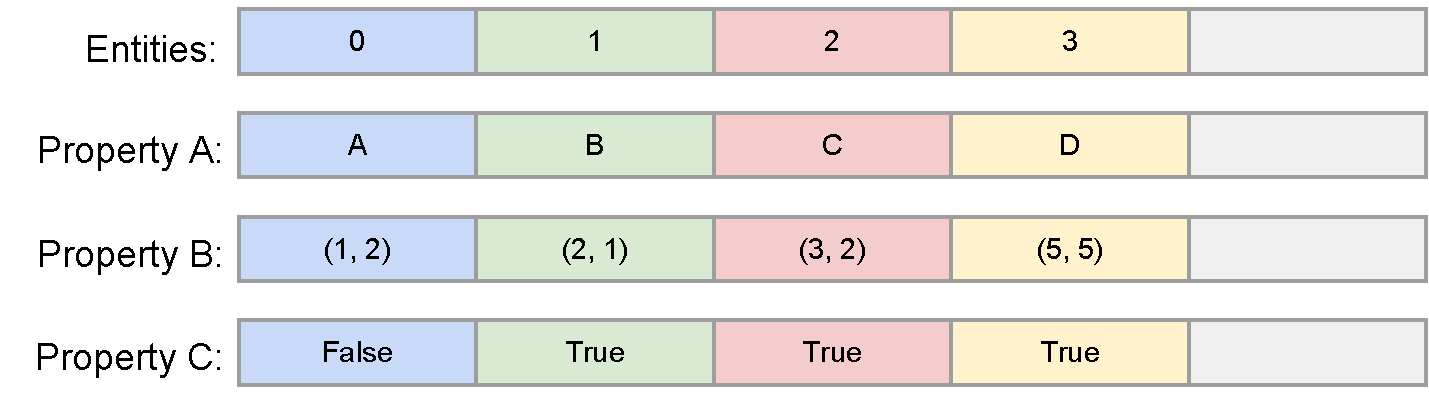
\includegraphics[width=0.7\linewidth]{img/tecnica/entityPropertyDOD}
%     % \caption{Modeling entities and their properties with \ac{dod} approach.}
%     \caption[Exemplo de entidades DOD]{Exemplo de entidades e suas propriedades seguindo o modelo de programação DOD.}
%     \label{fig:entityPropertyDOD}
% \end{figure}

Com objetivo de explanar como a organização dos pode impactar na utilização da memória cache, a Figura~\ref{fig:cache_register_clustering} apresenta dois trechos de códigos (lado esquerdo) e como este código impactaria na cache (lado direito). Ambos os códigos possuem a mesma funcionalidade, sendo somente a organização dos dados diferente. A Figura~\ref{fig:cache_register_clustering}~(a) representa a modelagem dos dados seguindo a abordagem \ac{aos} que é tradicionalmente utilizada na orientação a objetos (OOD).A Figura~\ref{fig:cache_register_clustering}~(b) representa a abordagem \ac{soa} que é utilizada no modelo orientado a dados (DOD).

\begin{figure}[bh]
    \subfigure[Array of Structures (AoS)]{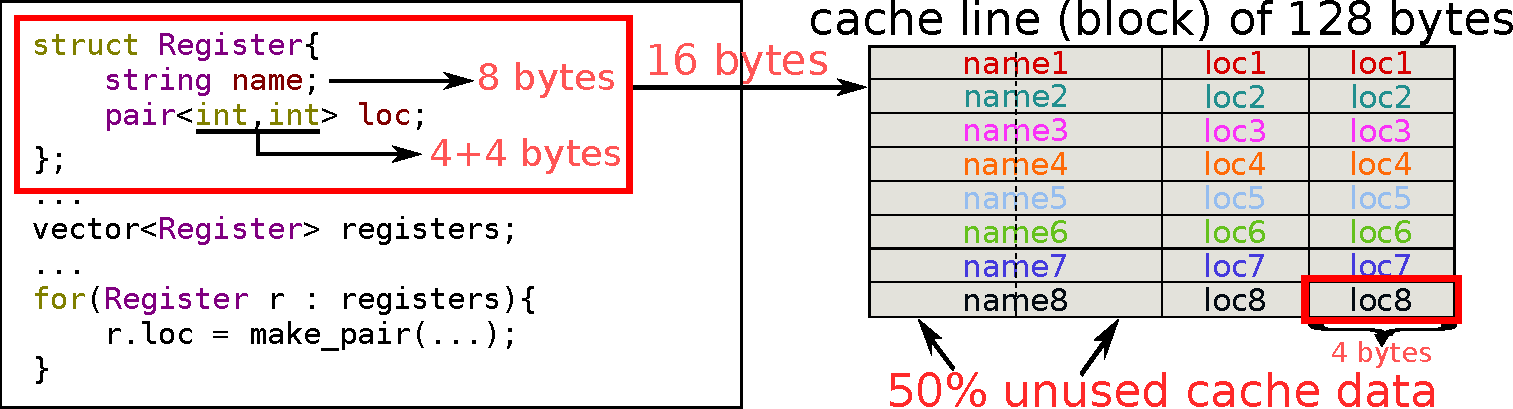
\includegraphics[width=\linewidth]{img/tecnica/cacheUtilizationRegisterClusterclassOOD}}
    % to break figure
    \subfigure[Structure of Arrays (SoA)]{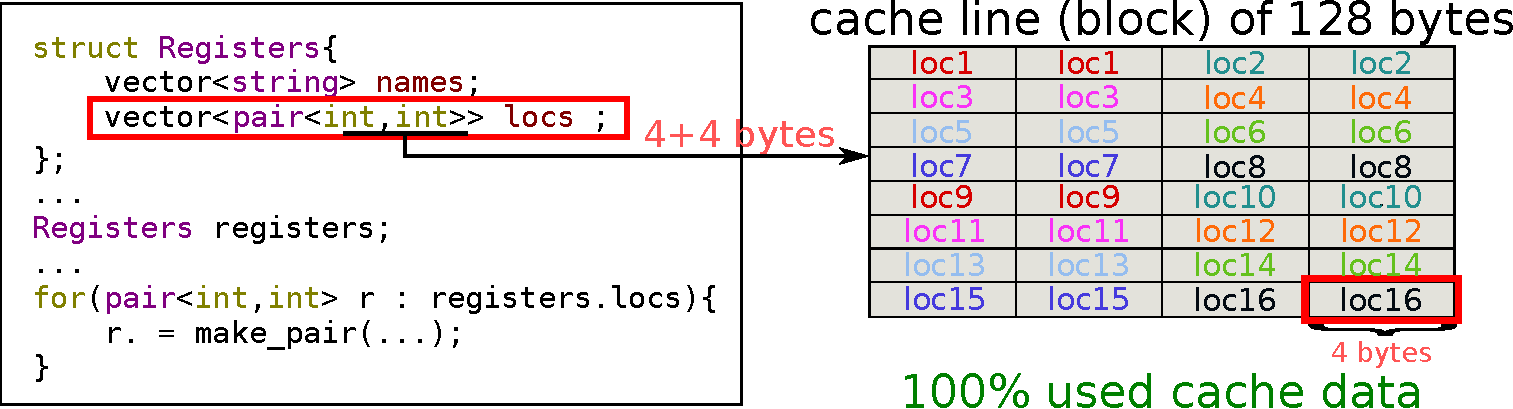
\includegraphics[width=\linewidth]{img/tecnica/cacheUtilizationRegisterClusterclassDOD}}
    \caption[Comparação da utilização da cache]{Comparação da utilização da cache para diferentes modelos de organização dos dados.}
    \label{fig:cache_register_clustering}
\end{figure}

Pode-se notar que no modelo \ac{ood}, quando ocorre um cache miss todo o objeto precisa ser recuperado para a cache. Ao recuperar todas as informações do objeto, desperdiça-se espaço com atributos/informações que não serão utilizadas na solução do problema. No exemplo da Figura~\ref{fig:cache_register_clustering}~(a) são carregados para a cache o nome dos registradores, porém, somente deseja-se alterar as posições dos registradores. Assim, $50\%$ dos dados recuperados por um cache miss são desperdiçados.



Utilizando-se o modelo \ac{dod}, Figura~\ref{fig:cache_register_clustering}~(b), quando um cache miss ocorre somente o vetor das propriedades necessárias é recuperado para a cache. Este fato implica em que atributos desnecessários para esta execução não sejam recuperados. Assim, a memória cache é preenchida somente com dados úteis.
Seguindo esta abordagem, o número de cache misses será menor e consequentemente o tempo de acesso aos dados da memória principal. Estes fatores possivelmente poderão reduzir o tempo total despendido por uma aplicação para executar determinada tarefa.



Para exemplificar a diferença entre os modelos \ac{ood} e \ac{dod} na modelagem dos dados, a Figura~\ref{fig:modelo_register_clustering} apresenta uma possível solução para o problema de clusterização de registradores seguindo estes dois modelos.
Na Figura Figura~\ref{fig:modelo_register_clustering}~(a) é apresentado a modelagem do problema com objetos. Nesta modelagem são necessárias duas classes: uma para representar os registradores (\textit{Register}) e outra para representas os clusters (\textit{Cluster}). Ambas as classes possuem dois atributos. A classe \textit{Cluster} possui a posição de seu centro e os registradores que pertencem a este cluster. A classe \textit{Register}, por sua vez, possui o nome e a posição do registrador.

\begin{figure}[ht]
    \centering
    \subfigure[OOD]{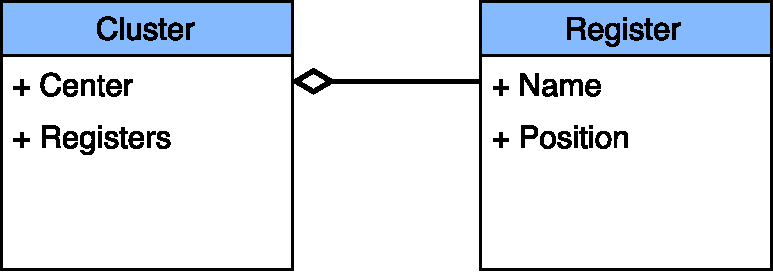
\includegraphics[width=0.5\linewidth]{img/tecnica/registerClusterclassOOD}}
    % to break figure
    \subfigure[DOD]{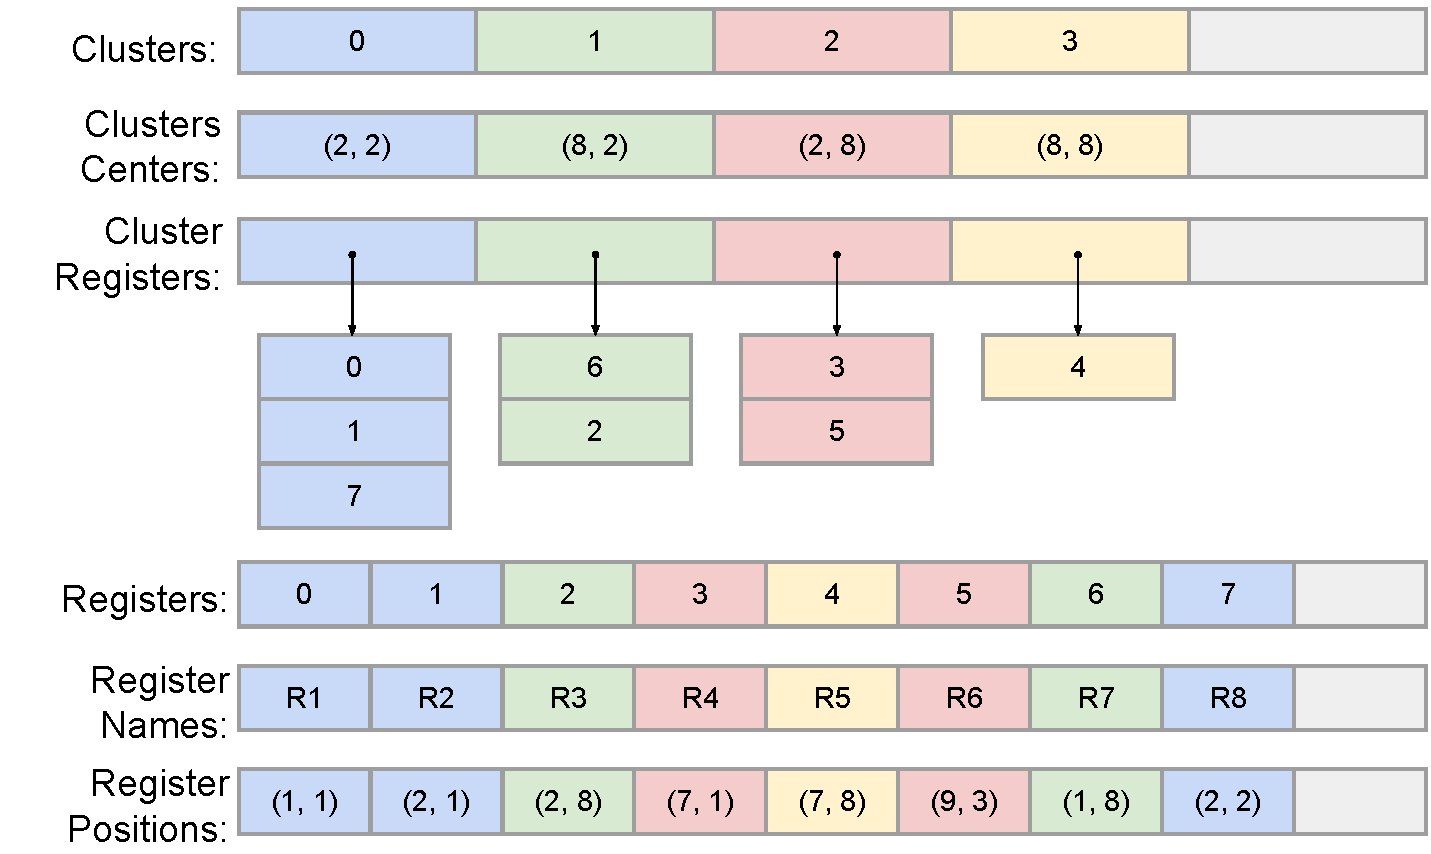
\includegraphics[width=0.8\linewidth]{img/tecnica/registerClusterclassDOD}}
    \caption{Modelagem dos dados para clusterização de registradores.}
    \label{fig:modelo_register_clustering}
\end{figure}


A Figura~\ref{fig:modelo_register_clustering}~(b) representa os mesmos dados da Figura~\ref{fig:modelo_register_clustering}~(a) porém, seguindo o modelo de programação \ac{dod}.
% Nesta figura cada cor representa uma instância que seria criada no modelo orientado a objetos. Os vetores \textit{Clusters} e \textit{Registers} armazenam contiguamente os indices dos objetos.
Nesta figura cada linha representa um vetor.
Cada atributo criado no modelo \ac{ood} é aqui representado por uma propriedades e é armazenada contiguamente em um único vetor.
Os vetores ``\textit{Clusters}'' e ``\textit{Registers}'' armazenam as entidades, sendo os demais vetores as propriedades destas entidades.
Estas propriedades serão agora recuperadas a partir do índice de uma entidade.
Por exemplo, a posição de um registrador $i$ é recuperada acessando o vetor ``\textit{Register Positions}'' na posição $i$.

Embora o modelo \ac{dod} possa reduzir o número de cache mmisses, seu conceito não é trivial de adotar, já que a maioria dos desenvolvedores de software estão acostumados a pensar nos relacionamentos dos objetos ao invés da organização de dados. Para usar eficientemente este modelo de programação, é necessário gerenciar os arrays de propriedades para garantir que os mesmos permaneçam contíguos à medida que novos dados são adicionados e/ou removidos. Um padrão de design chamado Sistema de Componente e Entidade (\textit{Entity-Component System}) pode ser adotado para lidar com esse problema~\cite{nystrom2014game}. Este padrão de projeto será descrito na seção a seguir.

\section{\textit{Entity-Component System}}
\label{sec:entity_component_system}

Esta Seção irá explanar os conceitos que são envolvidos no padrão de projetos \textit{Entity-Component System}.
Primeiramente serão explicados o que são Entidades e Componentes e como seriam relacionados com o padrão de projeto \ac{ood}.
Posteriormente, será abordado como gerenciar as entidades para que operações elementares sejam em tempo computacional constante.

\subsection{Entidades e Componentes}

O padrão de projeto \textit{Entity-Component System} consiste em decompor um problema em um conjunto de entidades e seus componentes~\cite{nystrom2014game}. As entidades são análogas aos objetos no modelo \ac{ood}, enquanto os componentes correspondem às suas propriedades (ou atributos). Neste trabalho, os componentes serão referenciados por propriedades para conformidade com o código fonte disponibilizado na plataforma GitHub. Diferentemente dos objetos, as entidades não são estruturas complexas, mas apenas identificadores únicos (IDs). Cada propriedade, por sua vez, é representada usando uma vetor de dados. O ID da entidade é usado para acessar suas propriedades nesses vetores. Por exemplo, a Figura~\ref{fig:entity_example} ilustra uma entidade com cinco propriedades, onde cada propriedade corresponde a um vetor e o ID da entidade é utilizado para acessar todos os vetores. Da mesma forma que as propriedades, cada uma dessas entidades é armazenada em um vetor contíguo.

\begin{figure}[ht]
    \centering
    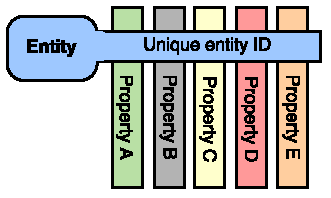
\includegraphics[width=0.5\linewidth]{img/tecnica/entity}
    % \caption{Example of entity with five properties. The entity id is used to access the information of all properties.}
    \caption[Exemplo de uma entidade]{Exemplo de uma entidade com cinco propriedades. O índice (ID) da entidade é utilizado para acessar as informações de todas as propriedades.}
    \label{fig:entity_example}
\end{figure}

\subsection{Sistema de Entidades}

O sistema de entidade é necessário para gerenciar o acessar as entidades e suas propriedades. Este sistema também é responsável por criar e destruir entidades, bem como gerenciar os vetores das propriedades ao alterar o número de entidades. Por exemplo, se uma entidade for criada ou destruída, o sistema da entidade deve assegurar de forma eficiente que todos os vetores permanecem contíguos na memória.

Além de gerenciar a criação e destruição de entidades, o sistema de entidade deve fornecer uma interface de acesso as entidades e suas propriedades com complexidade de tempo constante  ($\mathcal{O}(1)$). Para apresentar os algoritmos do sistema da entidade, vamos usar a notação descrita na Tabela~\ref{tab:notations}. Observe que $E_S$ e $P$ são vetores e, portanto, seus valores podem ser acessados através dos índices correspondentes. Por exemplo, $E_S(i)$ representa a entidade na i-ésima posição do vetor de entidades.

\begin{table}[!ht]
\centering
\caption{Notações utilizada no \textit{Entity-Component System} }
\label{tab:notations}
\resizebox{\linewidth}{!}{
\begin{tabular}{ c l }
\toprule[0.15em]
\textbf{Symbol}     & \textbf{Meaning}    \\ \midrule[0.1em]
$S$         & sistema de entidades $S$ \\
$e$         & entidade $e$ \\
$id_e$      & índice ($id$) da entidade $e$ \\
$E_S$       & vetor de entidades pertencente ao sistema de entidade $S$ \\
$E_S(i)$    & entidade armazenada na i-ésima posição do vetor $E$ \\
$\mathcal{P}_S$       & conjunto de propriedades associadas a um sistema de entidades $S$ \\
$P$         & vetor de propriedades $P$ \\
$P(j)$      & valor armazenado na j-ésima posição do vetor de propriedades $P$ \\ \bottomrule[0.15em]
% $C(e, e')$ & composition relationship between entities $e$ and $e'$ \\
% $A(e, e')$ & aggregation relationship between entities $e$ and $e'$ \\ \bottomrule[0.15em]
\end{tabular}
}
\end{table}

\simbolo{$S$}{sistema de entidades $S$}
\simbolo{$e$}{entidade $e$}
\simbolo{$id_e$}{índice ($id$) da entidade $e$}
\simbolo{$E_S$}{vetor de entidades pertencente ao sistema de entidade $S$}
\simbolo{$E_S(i)$}{entidade armazenada na i-ésima posição do vetor $E$}
\simbolo{$\mathcal{P}_S$}{conjunto de propriedades associadas a $S$}
\simbolo{$P$}{vetor de propriedades $P$}
\simbolo{$P(j)$}{valor armazenado na j-ésima posição de $P$}


O Algorítimo~\ref{alg:entityCreate} descreve como o sistema da entidade cria novas entidades. Quando uma nova entidade $ e $ é criada (linha 1), o sistema da entidade atribui a $ e $ um identificador $ id_e $ equivalente ao tamanho do vetor de entidades $ E_S $ (linha 2). Então a entidade $ e $ é inserida no final do vetor de entidades $ E_S $, chamando a função $ PUSH\_BACK $ (linha 3). Finalmente, para cada propriedade $P$ associada ao sistema da entidade $S$, um valor padrão é adicionado para a nova entidade $ e $ (linhas 4-6). Observe que o identificador de $ e $ ($ id_e $) é usado como um índice para acessar os vetores de propriedades.

\begin{algorithm}[ht]
%  \scriptsize
% \footnotesize
 \SetKwInOut{Input}{Input}\SetKwInOut{Output}{Output}
 \LinesNumbered
      \Input{Sistema de entidade $S$}
      \Output{Nova entidade $e$}
      $e \gets $ nova entidade\;
      $id_e \gets |E_S|$\;
      $PUSH\_BACK(E_S, e)$\;
      %$E(S) \gets E(S) \cup \{e\}$\;
      \ForEach{$P \in \mathcal{P}_S$}{
            $P(id_e) \gets$ valor padrão\;
      }
      \KwRet{$e$}\;
   \caption{ENTITY\_CREATE}
   \label{alg:entityCreate}
 \end{algorithm}

 O Algoritmo~\ref{alg:entityDestroy} apresenta as etapas de remoção de uma entidade. Dada uma entidade $ e $ para ser destruída, o sistema da entidade poderia simplesmente removê-lo do vetor de entidades. No entanto, remover um elemento do meio de um vetor contíguo tem uma complexidade de tempo de $\mathcal{O}(n)$, sendo $ n $ o número de entidades. Outra opção seria atribuir a entidade $ e $ como inválida, em vez de removê-la do vetor. No entanto, essa abordagem deixaria buracos no vetor de entidades, o que poderia degradar o desempenho do sistema da entidade.

  Em vez de remover a entidade $ e $ do vetor ou atribuí-la como inválida, o sistema de entidade substitui a entidade $e$ pela última entidade $e'$ do vetor de entidades (linhas 1-4). Em seguida, o último elemento deste vetor é removido ao chamar a função $ POP\_BACK $ (linha 5). Desta forma, o vetor de entidades permanece contíguo na memória e a operação de remoção é executada em~$\mathcal{O}(1)$. Depois de substituir $ e $ por $ e' $, o sistema de entidade faz o mesmo para os vetores de propriedades, substituindo os valores associados à entidade $ e $ por aqueles associados com a entidade $ e' $ (linhas 6-9). Por fim é retornado o sistema de entidades $S$ sem a entidade $e$.

 \begin{algorithm} [ht]
 %  \scriptsize
 % \footnotesize
  \SetKwInOut{Input}{Input}\SetKwInOut{Output}{Output}
  \LinesNumbered
       \Input{Sistema de entidade $S$, e entidade $e$ a ser removida}
       \Output{Sistema de entidade $S$ sem a entidade $e$}
         $n \gets |E_S|$\;
         $e' \gets E_S(n-1)$\;
         $E_S(id_e) \gets e'$\;
         $id_{e'} \gets id_e$\;
         $POP\_BACK(E_S)$\;
         \ForEach{$P \in \mathcal{P}_S$}{
             $P(id_e) \gets P(n-1)$\;
             $POP\_BACK(P)$\;
         }
         % $\mathcal{C} \gets \{C(e, e'') \mid e$ is composed by $e''\}$\;
         % \ForEach{$C(e, e'') \in \mathcal{C}$}{
         %     $DESTROY(C(e, e''))$\;
         %     $ENTITY\_DESTROY(S, e'')$\;
         % }
         % $\mathcal{A} \gets \{A(e, e'') \mid e$ is aggregated by $e''\}$\;
         % \ForEach{$A(e, e'') \in \mathcal{C}$}{
         %     $DESTROY(A(e, e''))$\;
         % }
         \KwRet{$S$}\;
    \caption{ENTITY\_DESTROY}
    \label{alg:entityDestroy}
  \end{algorithm}

  Em vez de usar relacionamentos hierárquicos (como \ac{ood}), o padrão de projeto \textit{Entity-Component System} representa relações entre as entidades por meio de composição e agregação. Uma composição representa uma relação de posse. Uma agregação, por sua vez, é simplesmente uma associação entre diferentes entidades, sem posse~\cite{gamma1995design}.
  % Figura \ref {} mostra exemplos de composição e agregações no contexto do design físico.
  Por exemplo, uma célula de circuito é composta por pinos, o que significa que, quando a célula é destruída, todos os seus pinos devem ser destruídos também. Por outro lado, a relação entre uma interconexão e seus pinos é simplesmente uma agregação. Como consequência, se uma interconexão é destruída, a relação também é destruída, mas todos os pinos permanecem no sistema da entidade.

  Esses relacionamentos podem ser adicionados à implementação do sistema de entidade (Algoritmos~\ref{alg:entityCreate} e~\ref{alg:entityDestroy}) como propriedades especiais. Desta forma, quando a propriedade é removida do vetor de propriedades (linha $ 8 $ do Algoritmo~\ref{alg:entityDestroy}), ele remove automaticamente o relacionamento. Além disso, se a propriedade é uma composição, serão removidas todas as entidades relacionadas.


% Com objetivo de mensurar quantitativamente o percentual de redução no número de cache misses e no tempo de execução, este trabalho irá analisar três tarefas de  Physical Design Automation.
% As subseções a seguir explanam como a organização dos dados
% -- ou --
% Este capítulo apresenta a proposta de organização dos dados para melhorar o desempenho de problemas de Physical Design Automation. Inicialmente, são discutidas as limitações do modelo de \ac{ood} e como o modelo de \ac{dod} pode sanar os mesmos. Em seguida, é discutido como o modelo \ac{dod} pode reduzir no número de cache misses. Por fim, são apresentados como podem ser aplicados os dois modelos (\ac{ood} e \ac{dod}) em três tarefas de Physical Design Automation.
%
% \section{Modelo de Programação Orientado a Objetos}
% \label{sec:modelo_orientado_objetos}
%
% Tipicamente, ferramentas de \ac{eda} são construídas utilizando o modelo de programação \ac{ood}.
% Este modelo decompõe o problema em objetos e mapeia estes objetos de mundo real para classes.
% Esses objetos são acessados através de uma interface bem definida e suas relações são representadas através da hierarquia, composição e agregação~\cite{booch2006object}.
% O modelo de programação \ac{ood} é popular porque geralmente há um mapeamento um-para-um entre os objetos do mundo real e seus objetos correspondentes no programa.
% Esta relação facilita a escrita e depuração do código.
%
%
% Para ilustrar os conceitos básicos aplicados no modelo de programação \ac{ood}, suponha que uma biblioteca de Physical Design precise ser desenvolvida.
% Esta biblioteca deverá solucionar uma ampla gama de problemas.
% Em seguida, assuma que um desenvolvedor de software deseja utilizar esta biblioteca para construir uma ferramenta que irá estimar o comprimento das interconexões (\textit{nets}) de um determinado circuito.
% A Figura~\ref{fig:circuito_exemplo} apresenta um exemplo de um circuito digital contendo quatro Nets e oito pinos.
%
%
% \begin{figure}[ht]
%     \centering
%     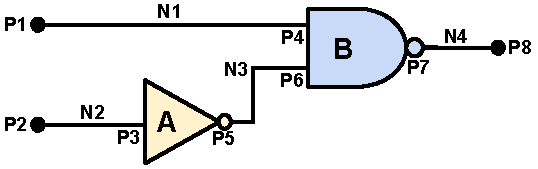
\includegraphics[width=0.7\linewidth]{img/tecnica/circuitExample}
%     % \caption{Combinational circuit portion with two logic gates (A and B), four nets (N1 to N4), and eight pins (P1 to P8).}
%     \caption[Fragmento de um circuito combinacional]{Fragmento de um circuito combinacional composto por duas portas lógicas (A e B), quatro nets (N1 a N4) e oito pinos (P1 a P8).}
%     \label{fig:circuito_exemplo}
% \end{figure}
%
% Um estimador de comprimento de interconexão deve ter acesso à informação de quais pinos pertencem a cada Net, bem como às posições dos pinos dentro do leiaute do circuito.
% A Figura~\ref{fig:classHierarchyOOD} ilustra uma possível decomposição para o problema de estimativa de comprimento de interconexão seguindo o modelo de programação \ac{ood}.
% Este diagrama é composto por dois módulos: \textit{Netlist} e \textit{Placemment}.
% O módulo \textit{Netlist} possui duas classes, \textit{Net} e \textit{Pin}, para descrever as interconexões do circuito e os pinos associados.
% Para a classe \textit{Pin}, este módulo caracteriza apenas o nome do pino e a rede a que ele pertence, sem qualquer informação de posicionamento.
% O módulo \textit{Placemment}, por sua vez, descreve as posições dos pinos.
% A seta entre as classes \textit{Pin} e \textit{Net} representam uma relação de agregação, o que significa que a interconeção possui uma referência aos seus pinos, enquanto um pino tem uma referência à sua interconeção proprietária.
% A seta entre as duas classes \textit{Pin} representa um relacionamento hierárquico, o que significa que a classe \textit{Pin} do módulo \textit{Placement} estende os atributos do pino do módulo \textit{Netlist}.
%
% \begin{figure}[ht]
%     \centering
%     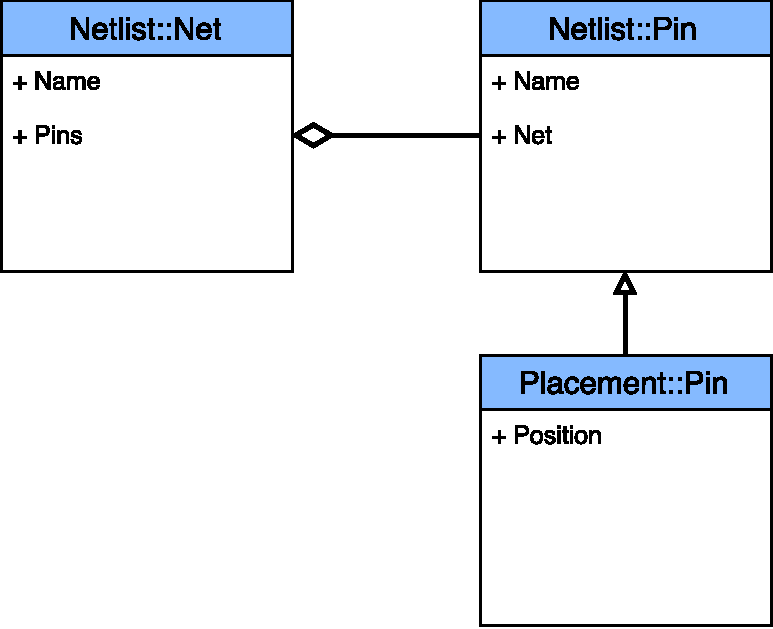
\includegraphics[width=0.5\linewidth]{img/tecnica/classHierarchyOOD}
%     % \caption{Class diagram to model wirelength estimation problem with \ac{ood} approach.}
%     \caption[Diagrama de classe com OOD]{Diagrama de classe para modelagem da estimativa do comprimento de uma intercenexão seguindo o modelo de programação \ac{ood}}
%     \label{fig:classHierarchyOOD}
% \end{figure}
%
% Embora possa ser fácil decompor um problema usando o modelo \ac{ood}, a implementação de um software, baseando-se apenas neste modelo de programação, pode levar a uma hierarquia de classes excessivamente complexa.
% Esta questão é particularmente crítica no desenvolvimento de uma biblioteca de software, pois é difícil prever, durante o design da biblioteca, como ela será realmente utilizada.
% Por exemplo, suponha que outro problema requer informações temporais sobre os pinos do circuito da Figura~\ref{fig:circuito_exemplo}.
% Seguindo o modelo de programação \ac{ood}, essas informações temporais podem ser adicionadas naturalmente criando um novo módulo chamado \textit{Timing} e uma nova classe \textit{Pin} (com atributos de temporização dos pinos) neste módulo.
% Por sua vez, esta nova classe deve também estender a classe \textit{Pin} do módulo \textit{Netlist}.
% Esta nova decomposição resulta na hierarquia de classes mostrada na Figura~\ref{fig:classHierarchyTimingOOD}.
%
% \begin{figure}[ht]
%     \centering
%     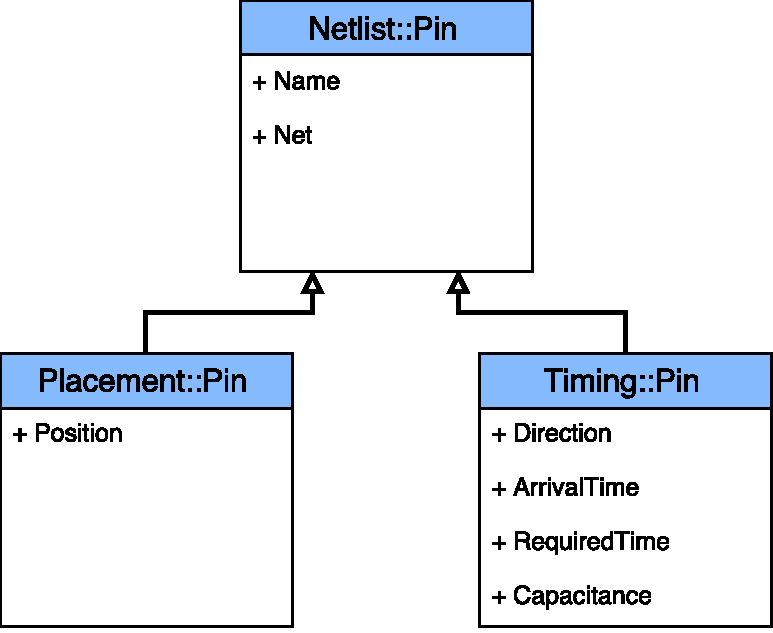
\includegraphics[width=0.5\linewidth]{img/tecnica/classHierarchyTimingOOD}
%     % \caption{Class diagram to model when pin timing information is added.}
%     \caption[Diagrama de classe de um pino]{Diagrama de classe de um pino com informações de posicionamento e temporais.}
%     \label{fig:classHierarchyTimingOOD}
% \end{figure}
%
%
% Agora, suponha que outro desenvolvedor queira usar nossa biblioteca de Physical Design para implementar um algoritmo de \ac{itdp}.
% Para fazer isso, este desenvolvedor irá precisar de uma nova classe \textit{Pin} com as informações de posicionamento e temporização.
% Em \ac{ood}, isso pode ser realizado através de herança múltipla, onde esta nova classe \textit{Pin} estende as classes \textit{Pin} de \textit{Placemment} e \textit{Timing}.
% No entanto, a herança múltipla não é suportada por todas as linguagens de programação, e mesmo quando suportada, não é recomendável porque pode levar a problemas de design~\cite{nystrom2014game}.
%
% Sem recorrer a herança múltipla, a solução consiste em criar uma nova classe \textit{Pin} que se estende do módulo \textit{Placement} ou \textit{Timing}, e repita o código da outra classe (que não foi estendida).
% Esta solução está apresentada na Figura~\ref{fig:classITDP}(a) e~\ref{fig:classITDP}(b).
% De qualquer forma, não existe uma maneira simples de reutilizar informações de posicionamento e tempo sem ocorrer replicação de código.
% A única opção restante é reunir todas as informações na classe \textit{Pin} do módulo \textit{Timing}, fazendo o mesmo estender o do módulo \textit{Placement}.
% Esta solução está ilustrada na Figura~\ref{fig:classITDP}(c).
% No entanto, nem sempre é necessário ter informações de posicionamento no módulo \textit{Timing}.
% Por exemplo, uma ferramenta analize de timing estática pode não precisar de informações de posicionamento durante etapas iniciais do projeto.
% Portanto, a adoção da última solução (Figura~\ref{fig:classITDP}(c)) levaria ao desperdício de memória, uma vez que informações desnecessárias seriam armazenadas.
%
% \begin{figure}[!ht]
%     \centering
%     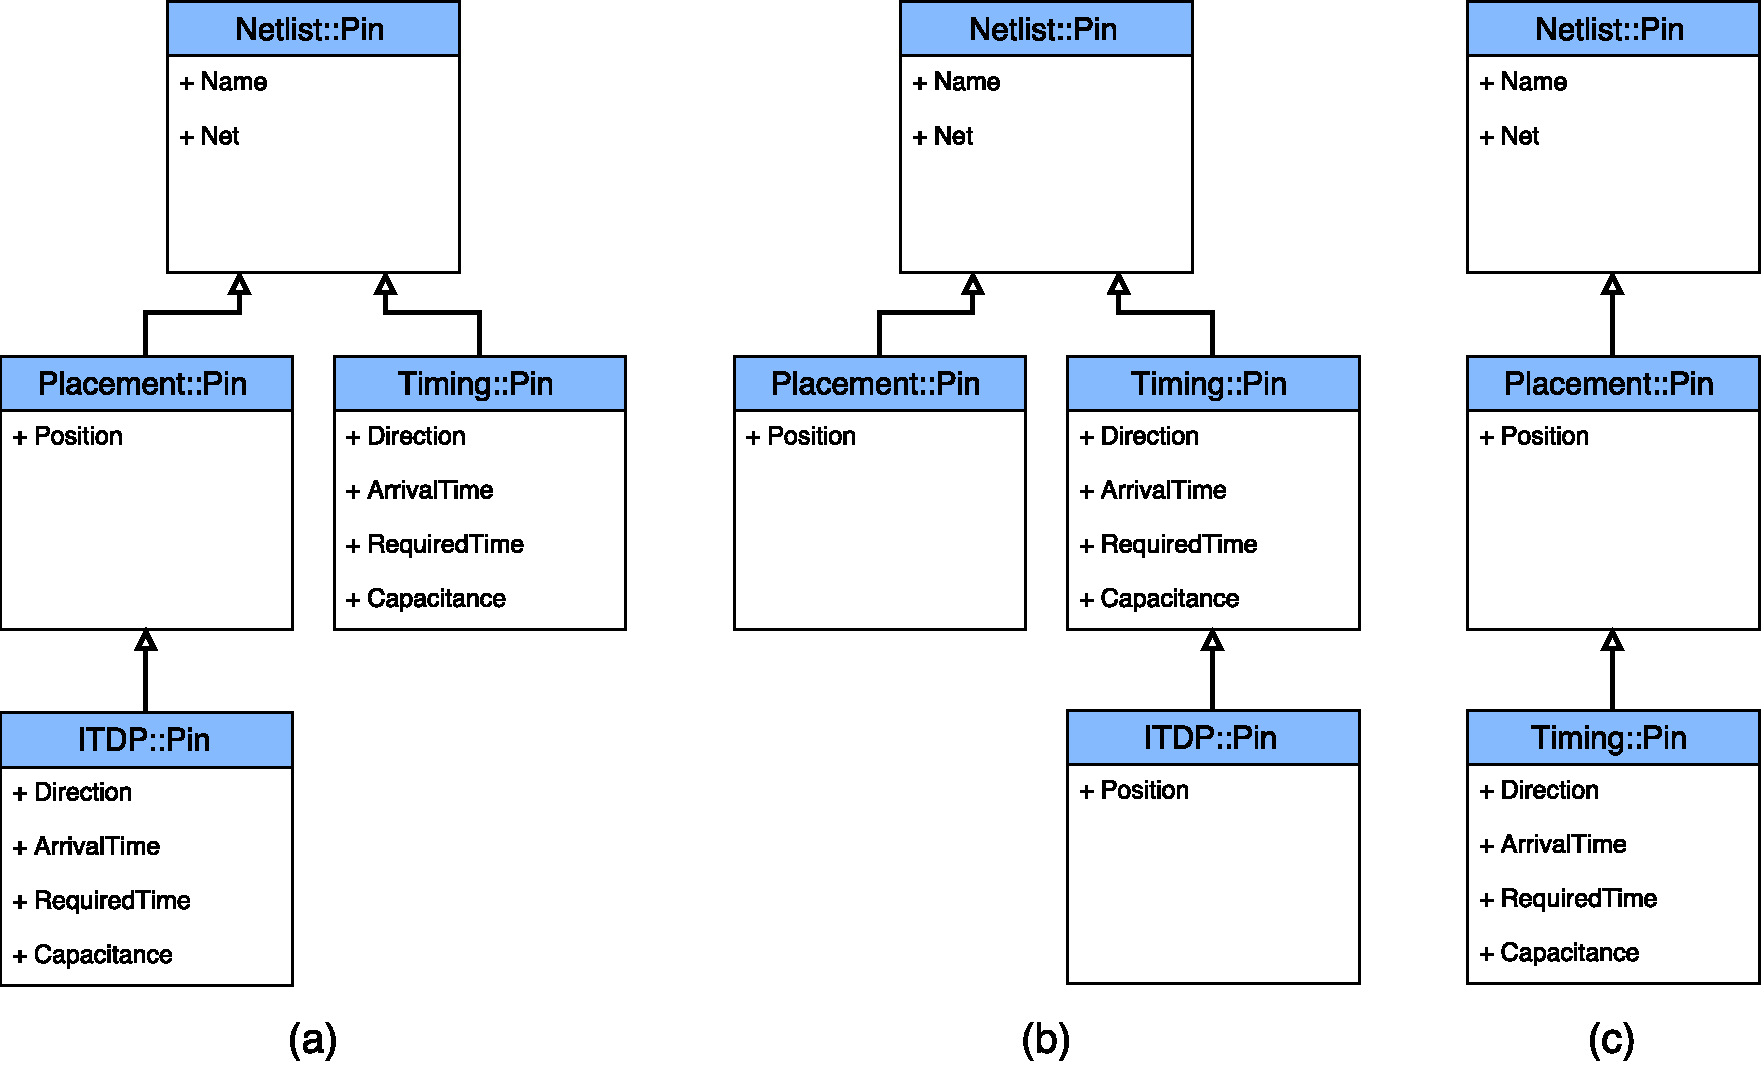
\includegraphics[width=\textwidth]{img/tecnica/ITDPsolutionOOD}
%     % \caption{Possible class hierarchy to support information of \textit{Timing} and \textit{Placement} for a timing-driven placement algorithm following \ac{ood} approach.}
%     \caption[Hierarquia de classes para suportar \textit{Timing} e \textit{Placement}]{Possível hierarquia de classes para suporte  informações de \textit{Timing} e \textit{Placement} para um algorítmo de \ac{itdp} seguindo o modelo de programação \ac{ood}.}
%     \label{fig:classITDP}
% \end{figure}




% \section{Modelo de Programação Orientado a Dados}
% \label{sec:modelo_orientado_dados}
%
% \section{Modelagem dos Dados para Physical Design}
% \label{sec:modelagem_physical_design}

% \subsection{Estudo de Caso A\@: Verificação dos Limites do Chip}
% \label{subsec:problema_A}

% \subsection{Estudo de Caso B\@: Estimativa de Interconexão}
% \label{subsec:problema_B}

% \subsection{Estudo de Caso C\@: Clusterização de Registradores}
% \label{subsec:problema_C}


% apresentar modelo de memoria
% apresentar como cache miss funciona
% apresentar ood
% apresentar limitação do ood
% apresentar dod
% apresentar entity system
% Discutir como o DOD reduz o numero de cache misses
% como aplicar o dod em problemas
%     Problema A - limites do chip
%         como seria modelado OOD
%         como seria modelado DOD
%     Problema B - interconexão
%         como seria modelado OOD
%         como seria modelado DOD
%     Problema C - cluster
%         como seria modelado OOD
%         como seria modelado DOD

    % proposta;
\chapter{Resultados Experimentais Preliminares}
\label{cap:resultados}

% Este capítulo apresenta os resultados experimentais obtidos por este trabalho. Inicialmente, ele descreve a infraestrutura experimental utilizada. Em seguida, analisa as três estratégias de legalização, no contexto de uma técnica de otimização incremental. Por fim, apresenta os resultados experimentais da avaliação da técnica proposta para legalização incremental.

\section{Infraestrutura experimental}
\label{sec:infraestrutura_experimental}

% Os experimentos realizados utilizaram o conjunto de benchmarks disponibilizados pela competição \textit{ICCAD 2015 CAD Contest (problem C: Incremental Timing-Driven Placement)} \cite{kim2015}, o qual inclui 8 circuitos que possuem entre 768k e 1,93M células, todos derivados de circuitos industriais. Para cada circuito, a infraestrutura da competição fornece um posicionamento inicial, o qual já está legalizado. Optou-se por utilizar tal infraestrutura pois a mesma disponibiliza circuitos com número de células compatível com circuitos contemporâneos. Além disso, tal infraestrutura é de acesso aberto, o que facilita a comparação experimental deste trabalho com futuros trabalhos que possivelmente serão realizados por terceiros.

% Todos os algoritmos apresentados neste capítulo foram implementados em C++. Para o desenvolvimento do protótipo com a técnica proposta, utilizou-se a implementação de R-tree disponível na biblioteca Boost \cite{boost}. Para fazer uso da R-tree é necessário definir dois de seus parâmetros: o grau da árvore e o algoritmo utilizado para a divisão de nodos durante a operação de inserção. Após alguns experimentos iniciais, não foi observada uma diferença significativa no tempo de execução das operações da R-tree ao variar o seu grau. Devido a isso, optou-se por utilizar uma árvore com grau 16. Por outro lado, o algoritmo de divisão de nodos utilizado tem impacto direto no tempo de execução da operação de inserção, assim como no tempo de execução das operações de busca subsequentes. Portanto, optou-se por utilizar o algoritmo denominado R*, que resulta em buscas espaciais mais rápidas, ao custo de um tempo de inserção um pouco maior.

% Todos os experimentos foram realizados em um computador Linux com quatro CPUs Intel\textsuperscript{\textregistered} Core\textsuperscript{\textregistered} i5-4460 @ 3,20 GHz e 32GB RAM. Os experimentos que avaliam o tempo de execução podem apresentar resultados diferentes em cada realização, devido a variações causadas pelo computador utilizado. Portanto, para aumentar a confiança estatística obtida pelos experimentos, os mesmos foram repetidos 10 vezes, o que resultou em 99\% de confiança estatística\footnote{A confiança estatística foi medida utilizando o teste t de Student para p=0,01.}. Como a confiança estatística obtida foi suficientemente alta, os experimentos não foram repetidos mais vezes.

\section{Comparação das estratégias de ...}



\chapter{Cronograma}
\label{cap:cronograma}

Este capítulo apresenta as atividades já concluídas até o momento da escrita deste documento, assim como as atividades pendentes que serão realizadas após o exame de qualificação.

\section{Atividades concluídas}

% \begin{itemize}
%     \item \textbf{C1}: Implementar o algoritmo proposto de legalização incremental;
%     \item \textbf{C2}: Implementar os trabalhos relacionados em legalização incremental propostos em \citeonline{chow2014cell} e \citeonline{popovych2014density};
%     \item \textbf{C3}: Avaliar o algoritmo proposto comparando-o com os trabalhos relacionados da atividade \textbf{C2};
%     \item \textbf{C4}: Implementar o algoritmo Abacus descrito em \citeonline{spindler2008abacus} para avaliar as estratégias de legalização final e iterativa;
%     \item \textbf{C5}: Comparar quantitativamente as três estratégias de legalização: final, iterativa e incremental;
%     \item \textbf{C6}: Submeter artigos às conferências ISVLSI 2016 (Qualis B1) e SBCCI 2016 (Qualis B1).
% \end{itemize}

\section{Atividades pendentes}

% \begin{itemize}
%     \item \textbf{P1}: Realizar as sugestões de melhoria do trabalho propostas pela banca no exame de qualificação;
%     \item \textbf{P2}: Apresentar o artigo no ISVLSI 2016;
%     \item \textbf{P3}: Apresentar o artigo no SBCCI 2016;
%     \item \textbf{P4}: Escrever a dissertação de mestrado;
%     \item \textbf{P5}: Preparar a apresentação e defender este trabalho de mestrado;
%     \item \textbf{P6}: Realizar as correções sugeridas pela banca durante a defesa;
%     \item \textbf{P7}: Entregar a versão final da dissertação de mestrado na Biblioteca Central da Universidade Federal de Santa Catarina.
% \end{itemize}

\section{Cronograma}

% A Figura \ref{tab:cronograma} apresenta o cronograma o previsto para realização deste trabalho de mestrado. Os meses de Junho a Agosto serão dedicados às correções sugeridas pela banca no exame de qualificação, assim como à apresentação do artigo aceito no ISVLSI 2016. Finalizando as correções, a dissertação será escrita a partir de Setembro, tendo sua finalização prevista em Novembro, quando inicará a preparação para a defesa, prevista para Dezembro. Por fim, os meses de Janeiro e Fevereiro são reservados para realizar as correções sugeridas pela banca na defesa e entrega do artigo na Biblioteca Central da Universidade Federal de Santa Catarina. Desta forma, a finalização deste trabalho de mestrado está dentro do prazo de 24 meses previsto pelo programa de Pós-Graduação em Ciência da Computação da Universidade Federal de Santa Catarina.

% \begin{table}[ht]
% \centering
% \resizebox{\textwidth}{!}{
% \begin{tabular}{@{}cccccccccc@{}}
% \toprule
%                                   & \textbf{Junho}         & \textbf{Julho}         & \textbf{Agosto}        & \textbf{Setembro}      & \textbf{Outubro}       & \textbf{Novembro}      & \textbf{Dezembro}      & \textbf{Janeiro}       & \textbf{Fevereiro}     \\ \midrule
% \multicolumn{1}{|c|}{\textbf{P1}} & \cellcolor[HTML]{FFFE65} & \cellcolor[HTML]{FFFE65}                      & \multicolumn{1}{c|}{\cellcolor[HTML]{FFFE65}} & \multicolumn{1}{c|}{}                         & \multicolumn{1}{c|}{}    & \multicolumn{1}{c|}{}                         & \multicolumn{1}{c|}{}                         & \multicolumn{1}{c|}{}    & \multicolumn{1}{c|}{}                         \\ \midrule
% \multicolumn{1}{|c|}{\textbf{P2}} & \multicolumn{1}{c|}{}    & \multicolumn{1}{c|}{\cellcolor[HTML]{FFFE65}} & \multicolumn{1}{c|}{}                         & \multicolumn{1}{c|}{}                         & \multicolumn{1}{c|}{}    & \multicolumn{1}{c|}{}                         & \multicolumn{1}{c|}{}                         & \multicolumn{1}{c|}{}    & \multicolumn{1}{c|}{}                         \\ \midrule
% \multicolumn{1}{|c|}{\textbf{P3}} & \multicolumn{1}{c|}{}    & \multicolumn{1}{c|}{}                         & \multicolumn{1}{c|}{}                         & \multicolumn{1}{c|}{\cellcolor[HTML]{FFFE65}} & \multicolumn{1}{c|}{}    & \multicolumn{1}{c|}{}                         & \multicolumn{1}{c|}{}                         & \multicolumn{1}{c|}{}    & \multicolumn{1}{c|}{}                         \\ \midrule
% \multicolumn{1}{|c|}{\textbf{P4}} & \multicolumn{1}{c|}{}    & \multicolumn{1}{c|}{}                         & \multicolumn{1}{c|}{}                         & \cellcolor[HTML]{FFFE65}                      & \cellcolor[HTML]{FFFE65} & \multicolumn{1}{c|}{\cellcolor[HTML]{FFFE65}} & \multicolumn{1}{c|}{}                         & \multicolumn{1}{c|}{}    & \multicolumn{1}{c|}{}                         \\ \midrule
% \multicolumn{1}{|c|}{\textbf{P5}} & \multicolumn{1}{c|}{}    & \multicolumn{1}{c|}{}                         & \multicolumn{1}{c|}{}                         & \multicolumn{1}{c|}{}                         & \multicolumn{1}{c|}{}    & \cellcolor[HTML]{FFFE65}                      & \multicolumn{1}{c|}{\cellcolor[HTML]{FFFE65}} & \multicolumn{1}{c|}{}    & \multicolumn{1}{c|}{}                         \\ \midrule
% \multicolumn{1}{|c|}{\textbf{P6}} & \multicolumn{1}{c|}{}    & \multicolumn{1}{c|}{}                         & \multicolumn{1}{c|}{}                         & \multicolumn{1}{c|}{}                         & \multicolumn{1}{c|}{}    & \multicolumn{1}{c|}{}                         & \multicolumn{1}{c|}{}                         & \cellcolor[HTML]{FFFE65} & \multicolumn{1}{c|}{\cellcolor[HTML]{FFFE65}} \\ \midrule
% \multicolumn{1}{|c|}{\textbf{P7}} & \multicolumn{1}{c|}{}    & \multicolumn{1}{c|}{}                         & \multicolumn{1}{c|}{}                         & \multicolumn{1}{c|}{}                         & \multicolumn{1}{c|}{}    & \multicolumn{1}{c|}{}                         & \multicolumn{1}{c|}{}                         & \multicolumn{1}{c|}{}    & \multicolumn{1}{c|}{\cellcolor[HTML]{FFFE65}} \\ \bottomrule
% \end{tabular}
% }
% \caption{Cronograma previsto para realização do trabalho de mestrado}
% \label{tab:cronograma}
% \end{table}
    % cronograma de desenvolvimento das atividades previstas, incluindo provável mês e ano da defesa;



% \chapter{Introdução}
\label{cap:introducao}
    % evolução da tecnologia -> transistores menores
    % circuitos modernos muito grande grandes -> ferramentas de EDA
    % eletrônica de consumo -> tempo limitado para projeto de um circuito
    % é benéfico a redução de tempo na execução dos algoritmos sem perda da qualidade da solução
    % memória representa gargalo -> explorar a localidade na cache
    %
    % uma possível solução que não altera a qualidade da solução é o melhor armazenamento dos dados

A evolução da tecnologia de fabricação de \acp{ic} vem permitindo uma redução drástica e contínua das dimensões dos transistores.
O consequente aumento de densidade permite a fabricação de \acp{ic} com um número cada vez maior de transistores, podendo chegar a milhões de transistores.
Além disso, os circuitos contemporâneos devem respeitar uma ampla gama de restrições, sejam elas de atraso, potência e\@/\@ou área.
Adicionalmente, o processo de projeto e fabricação possui um tempo limitado para que um novo eletronico possa garantir o mercado.
Portanto, as Ferramentas de \ac{eda} são obrigatórias no design de \acp{ic} modernos.




ferramentas seguem um fluxo de projeto
explicar o fluxo
varias etapas do fluxo podem voltar
dados das etapas podem ser reutilizados
é benefico uma melhor organização dos dados


Essas ferramentas de \ac{eda} devem tratar um grande volume de dados em um curto período de tempo. Portanto, essas ferramentas de \ac{eda} devem empregar otimizações de software, como o uso de melhores estruturas de dados, paralelização e exploração de local de cache.

modelagem dos dados deve ser ótima para diversas relações
OOD pode gerar uma hierarquia muito complexa e problemas sem solução (a não ser replicação do código)








este trabalho avalia o impacto da exploração da localidade do cache no agrupamento de registros.


\section{Justificativa}
    o que a literatura não fez
    Portanto, é desejável o desenvolvimento ... sobretudo uma comparação que faça uso de uma infraestrutura realista.

\section{Objetivos e Contribuições Pretendidas}
        Objetivo
            Este trabalho tem como objetivo a avaliação quantitativa do impacto de diferentes
        Objetivos específicos

        Contribuições científicas e tecnológicas
            avaliação quantitativamente do desempenho causado pela modelagem dos dados em três tarefas da síntese física
            Resultados experimentais utilizando uma infraestrutura baseada em circuitos industriais,

\section{Metodologia}
        Implementar versões de problemas
        avaliar quantitativamente o número de cache misses
        avaliar quantitativamente o tempo de execução

\section{Limitações(escopo) deste trabalho}
        somente 3 problemas avaliados
        somente uma arquitetura de processador e cache
        paralelização com um chunk único

\section{Organização deste trabalho}

% \input{capitulos/conceitos_fundamentais}
% \input{capitulos/formulacao_problema}
% \chapter{Trabalhos correlatos}
\label{cap:trabalhos_correlatos}

% Este capítulo apresenta os principais trabalhos correlatos no contexto do problema de legalização. Inicialmente, são revisados os principais algoritmos de legalização completa. Em seguida, são descritos os principais algoritmos propostos para resolver o problema de legalização incremental. É importante ressaltar que este capítulo não faz uma análise exaustiva dos algoritmos de legalização, mas busca apresentar os trabalhos mais relevantes relacionados às diferentes abordagens utilizadas para resolver o problema.

% \section{Trabalhos correlatos em legalização completa}

% % !TEX root = ../dissertacao.tex
\acresetall{}
\chapter{Explorando a localidade dos dados em Physical Design Automation}
\label{cap:tecnica_proposta}

Este capítulo apresenta a proposta de organização dos dados para melhorar o desempenho de tarefas de Physical Design Automation.
Inicialmente será revisado alguns conceitos básicos de acesso a memoria principal para recuperação dos dados.
Em seguida, serão discutidas as limitações do modelo \ac{ood} e como o modelo Orientado a Dados (DOD) pode sanar os mesmos.
% Por fim, será apresentado como aplicar os dois modelos (OOD e DOD) em três tarefas de Physical Design.
Por fim, na Seção~\ref{sec:entity_component_system}, será apresentado um padrão de projeto para facilitar o acesso as dados organizados segundo modelo \ac{dod}.

A arquitetura de memória de computadores modernos é tipicamente hierárquica como mostrado na Figura~\ref{fig:memoryHierarchy}. Observe que os níveis mais baixos na hierarquia (por exemplo, disco rígido e memória principal) têm maior capacidade, mas possuem maior latência. Por outro lado, os níveis mais altos (por exemplo, memória cache e registradores da CPU) são rápidos, mas possuem capacidade limitada. Quando um determinado programa precisa um dado, e o mesmo não se encontra nos registradores da CPU, será realizado uma busca por este dado nos níveis mais altos da hierarquia da  cache. Quando os dados não são encontrados em algum dos níveis de cache, dizemos que ocorreu um \textbf{cache miss}. Quando um cache miss ocorre, os dados são acessados no nível inferior da hierarquia. No pior caso, este dado será recuperado do disco rígido e levado por todos os níveis da hierarquia. Quando o dado buscado é recuperado para a cache de mais alto nível e posteriormente armazenado num registrador da CPU, o programa que estava acessando os dados volta a executar. Caso que esses dados forem necessários novamente, e o bloco da cache não tenha sido sobrescrito, eles estarão disponível na cache e sua busca nos níveis da cache resultará em \textbf{cache hit}~\cite{patterson2013computer}.

\begin{figure}[ht]
    \centering
    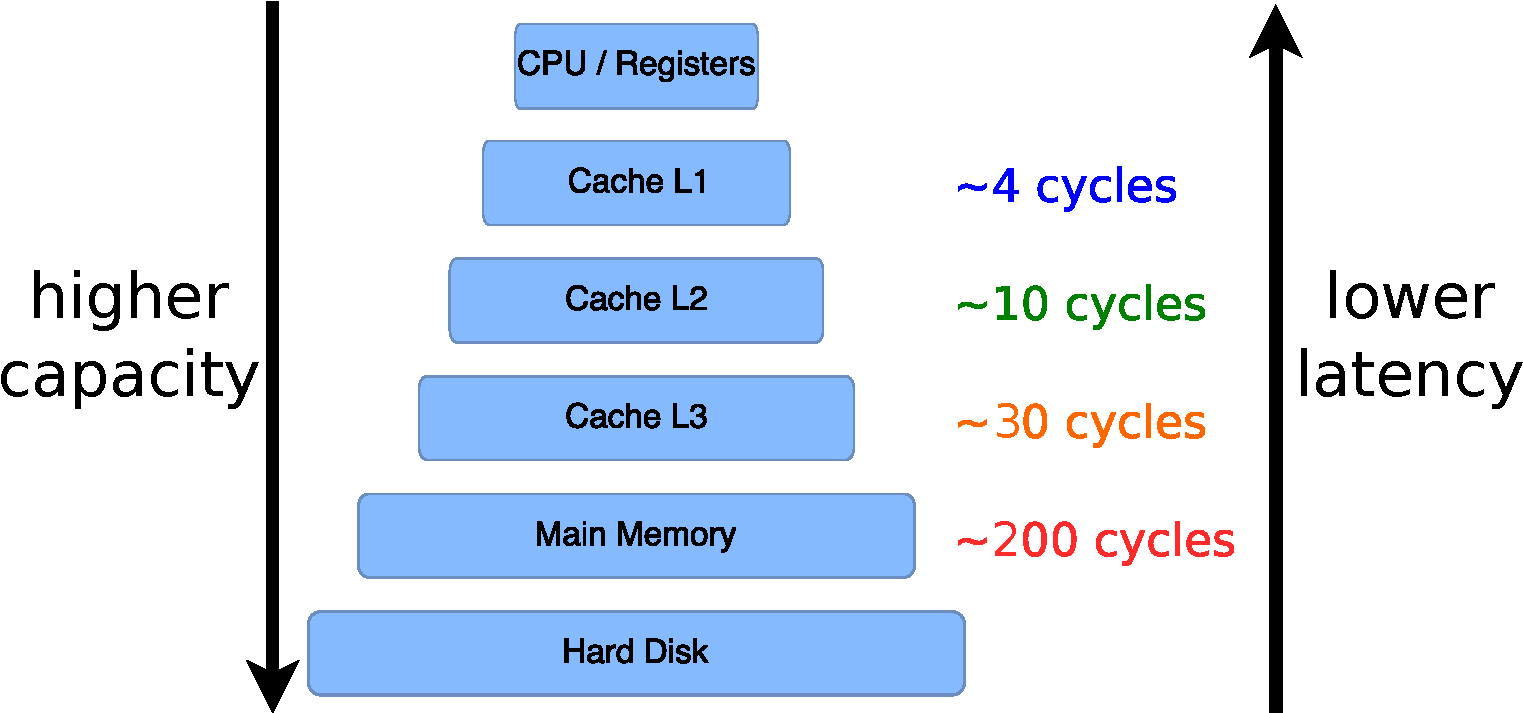
\includegraphics[width=0.7\linewidth]{img/tecnica/memoryHierarchy}
    % \caption{Hierarchy of memory present in modern computers. The hierarchy is compose by hard disk, main memory, three levels of cache and CPU registers. Adapted from~\cite{patterson2013computer}.}
    \caption[Hierarquia de memória]{Hierarquia de memória presente em computadores modernos. A hierarquia é composta por disco rígido, memória principal, três níveis de cache e registradores. Adaptada de~\cite{patterson2013computer}.}
    \label{fig:memoryHierarchy}
\end{figure}

A localidade espacial da cache (\textit{cache spatial locality}) é uma propriedade importante dos sistemas hierárquicos de memória. Esta propriedade afirma que a probabilidade de acessar um recurso da memória é maior se um recurso próximo já foi referenciado~\cite{patterson2013computer}. O sistema de cache explora esta propriedade armazenando os dados em blocos (\textit{cache blocks}). Sempre que algum dado é acessado a partir da memória principal, ele é recuperado para a cache juntamente com outros dados que estavam armazenados próximos a ele. Desta forma, se os dados próximos forem acessados posteriormente, resultarão em cache hits.

É possível explorar ainda mais a localidade espacial do cache, mudando a forma como os dados são organizados em um determinado software mesmo não possuindo nenhuma informação de qual será a organização e tamanho da cache.
Isto é possível uma vez que ao armazenar dados de uma mesma categoria de forma contígua estamos aumentando a probabilidade de um acesso gerar um cache hit.

Por exemplo, um algoritmo de Clusterização de Registradores executa operações em todas as posições dos registradores de um circuito.
Ao armazenar todas as posições dos registradores em um único vetor contíguo, este algoritmo irá necessitar de um número inferior de cache misses para recuperar todos os dados.
Como consequência, o tempo de acesso a dados é reduzido e o desempenho do software é melhorado. Esta organização de dados nem sempre é eficientemente feita pelo modelo de programação tradicional~\ac{ood}.
Neste modelo de programação, os dados são armazenados agrupando todas as informações de um mesmo objeto num único registro.
Observe que com esta abordagem, quando os objetos são recuperados para a cache, alguns dados inúteis (atributos do objeto) são carregados juntos. Portanto, a cache é desperdiçado com dados que provavelmente não serão utilizados pelo algoritmo.

Uma alternativa para o modelo de \ac{ood} é o modelo de programação \ac{dod}. Este modelo tem como enfoque a forma como os dados são organizados na memória.
% A Figura~\ref{fig:entityPropertyDOD} mostra um exemplo sobre como modelar os dados usando este modelo de programação.
Enquanto no modelo \ac{ood} utiliza objetos complexos e seus atributos para representar os objetos do mundo real, o modelo \ac{dod} representa os dados do mundo real como entidades e suas propriedades (atributos).
Cada entidade é simplesmente um índice. Este índice é utilizado para acessar suas propriedades.
Assim, cada propriedade pode ser armazenada num único vetor contíguo na memória.
% Por exemplo, na Figura~\ref{fig:entityPropertyDOD}, o vetor de entidades armazenam todos os índices das entidade, enquanto os outros vetores armazenam suas propriedades, as quais podem ser acessadas usando os índices do vetor de entidades.
Ao organizar os dados dessa forma, quando um algoritmo precisa apenas de uma propriedade (por exemplo a posição dos registradores) ele pode recuperar somente o vetor que contem estes dados.
Desta forma, não são recuperados dados desnecessários o que acarreta numa maior localidade espacial da cache.

% \begin{figure}[ht]
%     \centering
%     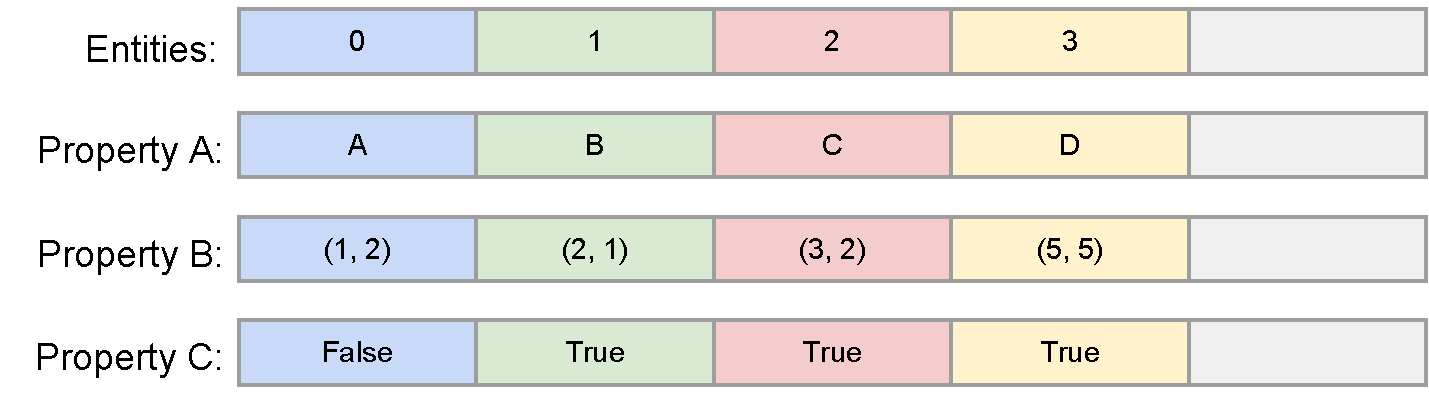
\includegraphics[width=0.7\linewidth]{img/tecnica/entityPropertyDOD}
%     % \caption{Modeling entities and their properties with \ac{dod} approach.}
%     \caption[Exemplo de entidades DOD]{Exemplo de entidades e suas propriedades seguindo o modelo de programação DOD.}
%     \label{fig:entityPropertyDOD}
% \end{figure}

Com objetivo de explanar como a organização dos pode impactar na utilização da memória cache, a Figura~\ref{fig:cache_register_clustering} apresenta dois trechos de códigos (lado esquerdo) e como este código impactaria na cache (lado direito). Ambos os códigos possuem a mesma funcionalidade, sendo somente a organização dos dados diferente. A Figura~\ref{fig:cache_register_clustering}~(a) representa a modelagem dos dados seguindo a abordagem \ac{aos} que é tradicionalmente utilizada na orientação a objetos (OOD).A Figura~\ref{fig:cache_register_clustering}~(b) representa a abordagem \ac{soa} que é utilizada no modelo orientado a dados (DOD).

\begin{figure}[bh]
    \subfigure[Array of Structures (AoS)]{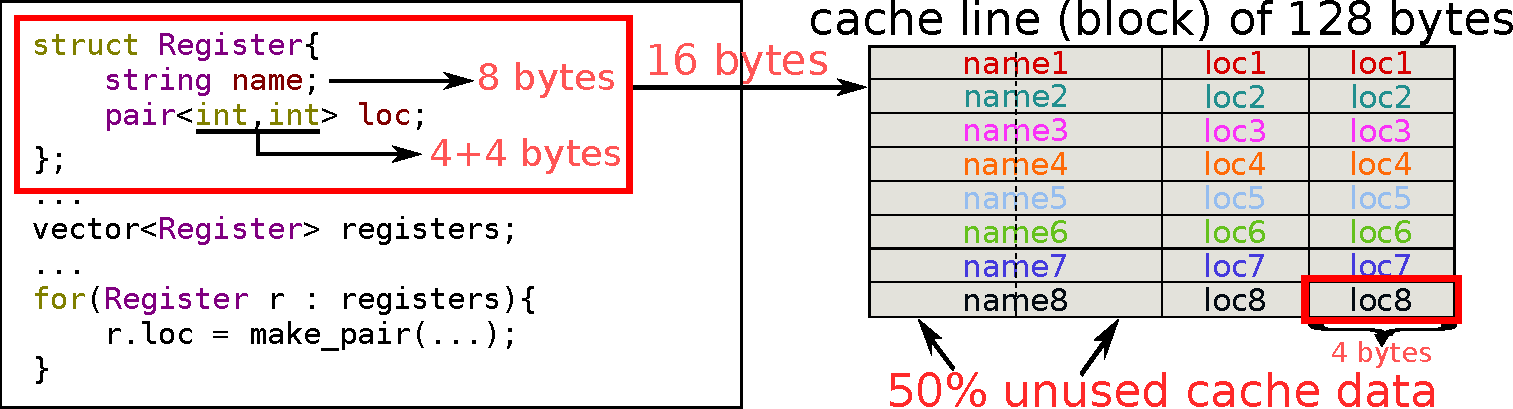
\includegraphics[width=\linewidth]{img/tecnica/cacheUtilizationRegisterClusterclassOOD}}
    % to break figure
    \subfigure[Structure of Arrays (SoA)]{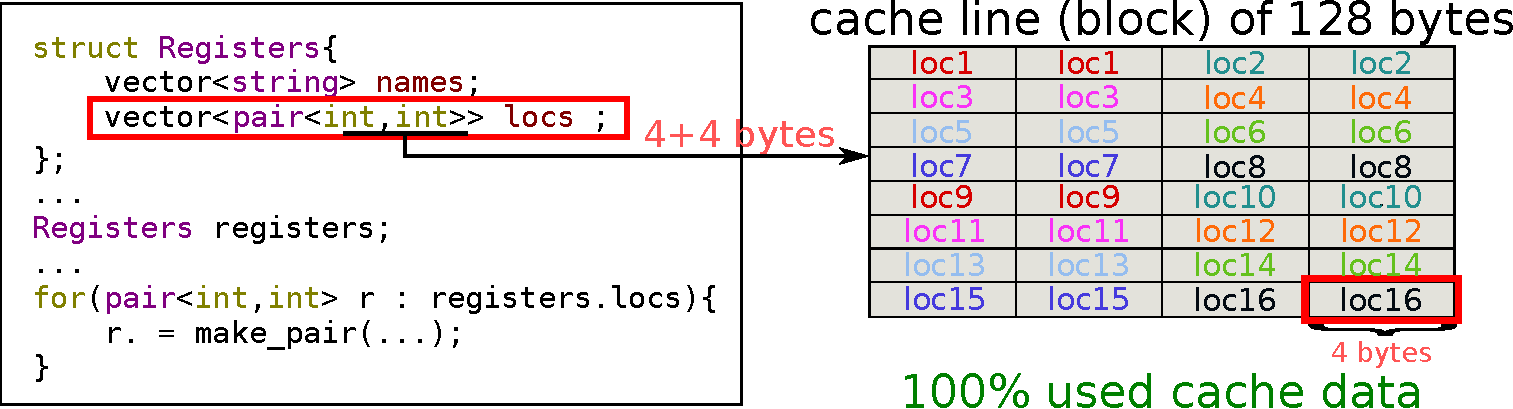
\includegraphics[width=\linewidth]{img/tecnica/cacheUtilizationRegisterClusterclassDOD}}
    \caption[Comparação da utilização da cache]{Comparação da utilização da cache para diferentes modelos de organização dos dados.}
    \label{fig:cache_register_clustering}
\end{figure}

Pode-se notar que no modelo \ac{ood}, quando ocorre um cache miss todo o objeto precisa ser recuperado para a cache. Ao recuperar todas as informações do objeto, desperdiça-se espaço com atributos/informações que não serão utilizadas na solução do problema. No exemplo da Figura~\ref{fig:cache_register_clustering}~(a) são carregados para a cache o nome dos registradores, porém, somente deseja-se alterar as posições dos registradores. Assim, $50\%$ dos dados recuperados por um cache miss são desperdiçados.



Utilizando-se o modelo \ac{dod}, Figura~\ref{fig:cache_register_clustering}~(b), quando um cache miss ocorre somente o vetor das propriedades necessárias é recuperado para a cache. Este fato implica em que atributos desnecessários para esta execução não sejam recuperados. Assim, a memória cache é preenchida somente com dados úteis.
Seguindo esta abordagem, o número de cache misses será menor e consequentemente o tempo de acesso aos dados da memória principal. Estes fatores possivelmente poderão reduzir o tempo total despendido por uma aplicação para executar determinada tarefa.



Para exemplificar a diferença entre os modelos \ac{ood} e \ac{dod} na modelagem dos dados, a Figura~\ref{fig:modelo_register_clustering} apresenta uma possível solução para o problema de clusterização de registradores seguindo estes dois modelos.
Na Figura Figura~\ref{fig:modelo_register_clustering}~(a) é apresentado a modelagem do problema com objetos. Nesta modelagem são necessárias duas classes: uma para representar os registradores (\textit{Register}) e outra para representas os clusters (\textit{Cluster}). Ambas as classes possuem dois atributos. A classe \textit{Cluster} possui a posição de seu centro e os registradores que pertencem a este cluster. A classe \textit{Register}, por sua vez, possui o nome e a posição do registrador.

\begin{figure}[ht]
    \centering
    \subfigure[OOD]{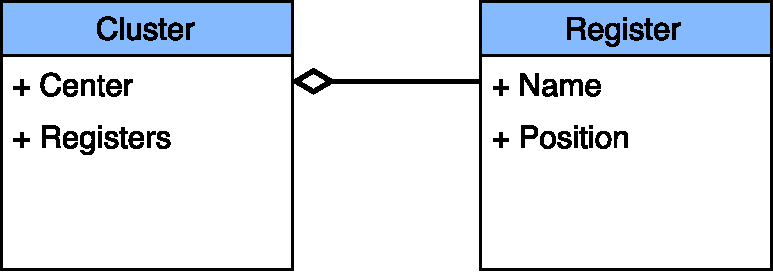
\includegraphics[width=0.5\linewidth]{img/tecnica/registerClusterclassOOD}}
    % to break figure
    \subfigure[DOD]{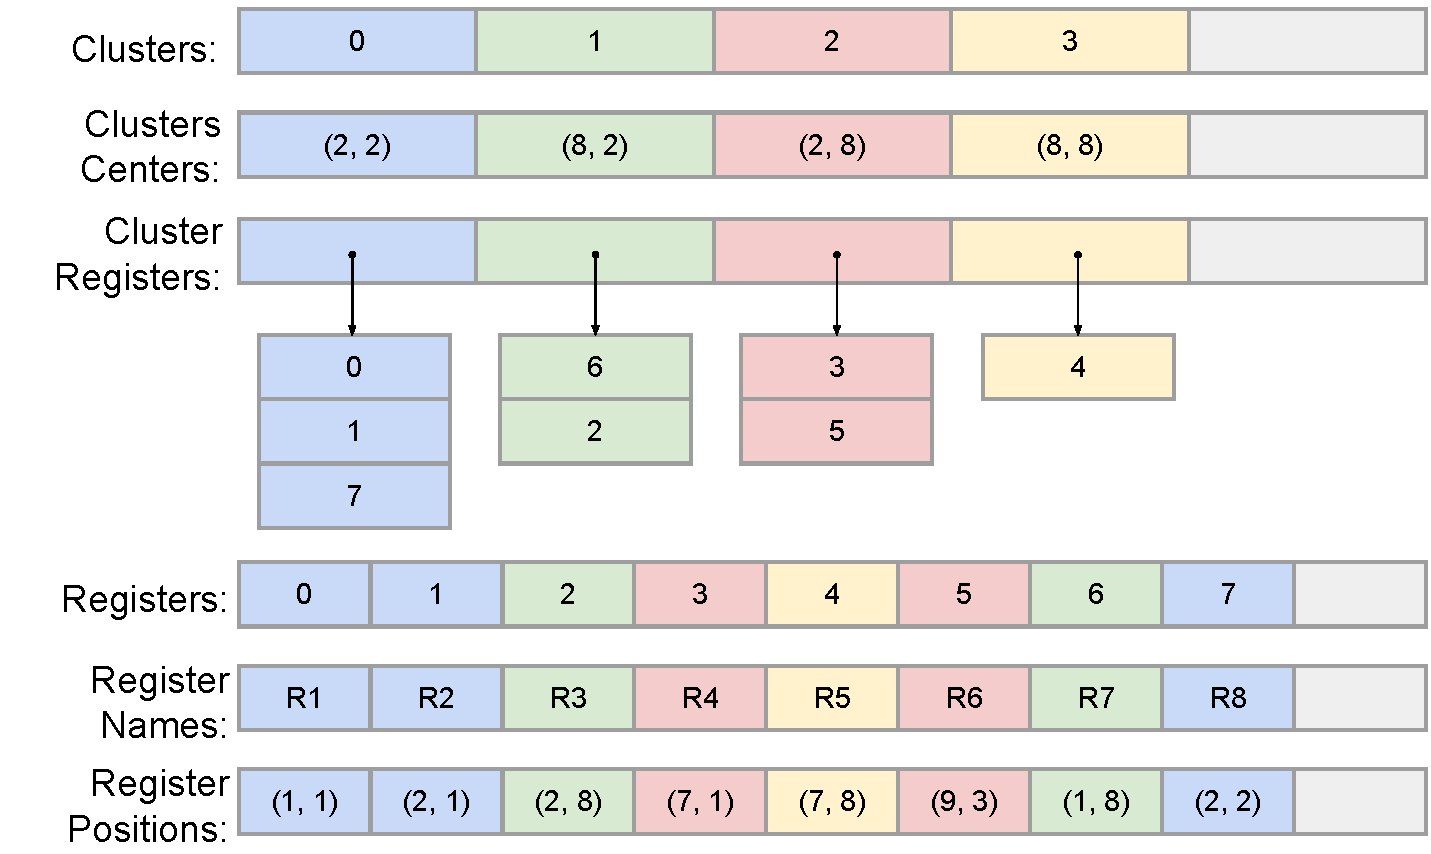
\includegraphics[width=0.8\linewidth]{img/tecnica/registerClusterclassDOD}}
    \caption{Modelagem dos dados para clusterização de registradores.}
    \label{fig:modelo_register_clustering}
\end{figure}


A Figura~\ref{fig:modelo_register_clustering}~(b) representa os mesmos dados da Figura~\ref{fig:modelo_register_clustering}~(a) porém, seguindo o modelo de programação \ac{dod}.
% Nesta figura cada cor representa uma instância que seria criada no modelo orientado a objetos. Os vetores \textit{Clusters} e \textit{Registers} armazenam contiguamente os indices dos objetos.
Nesta figura cada linha representa um vetor.
Cada atributo criado no modelo \ac{ood} é aqui representado por uma propriedades e é armazenada contiguamente em um único vetor.
Os vetores ``\textit{Clusters}'' e ``\textit{Registers}'' armazenam as entidades, sendo os demais vetores as propriedades destas entidades.
Estas propriedades serão agora recuperadas a partir do índice de uma entidade.
Por exemplo, a posição de um registrador $i$ é recuperada acessando o vetor ``\textit{Register Positions}'' na posição $i$.

Embora o modelo \ac{dod} possa reduzir o número de cache mmisses, seu conceito não é trivial de adotar, já que a maioria dos desenvolvedores de software estão acostumados a pensar nos relacionamentos dos objetos ao invés da organização de dados. Para usar eficientemente este modelo de programação, é necessário gerenciar os arrays de propriedades para garantir que os mesmos permaneçam contíguos à medida que novos dados são adicionados e/ou removidos. Um padrão de design chamado Sistema de Componente e Entidade (\textit{Entity-Component System}) pode ser adotado para lidar com esse problema~\cite{nystrom2014game}. Este padrão de projeto será descrito na seção a seguir.

\section{\textit{Entity-Component System}}
\label{sec:entity_component_system}

Esta Seção irá explanar os conceitos que são envolvidos no padrão de projetos \textit{Entity-Component System}.
Primeiramente serão explicados o que são Entidades e Componentes e como seriam relacionados com o padrão de projeto \ac{ood}.
Posteriormente, será abordado como gerenciar as entidades para que operações elementares sejam em tempo computacional constante.

\subsection{Entidades e Componentes}

O padrão de projeto \textit{Entity-Component System} consiste em decompor um problema em um conjunto de entidades e seus componentes~\cite{nystrom2014game}. As entidades são análogas aos objetos no modelo \ac{ood}, enquanto os componentes correspondem às suas propriedades (ou atributos). Neste trabalho, os componentes serão referenciados por propriedades para conformidade com o código fonte disponibilizado na plataforma GitHub. Diferentemente dos objetos, as entidades não são estruturas complexas, mas apenas identificadores únicos (IDs). Cada propriedade, por sua vez, é representada usando uma vetor de dados. O ID da entidade é usado para acessar suas propriedades nesses vetores. Por exemplo, a Figura~\ref{fig:entity_example} ilustra uma entidade com cinco propriedades, onde cada propriedade corresponde a um vetor e o ID da entidade é utilizado para acessar todos os vetores. Da mesma forma que as propriedades, cada uma dessas entidades é armazenada em um vetor contíguo.

\begin{figure}[ht]
    \centering
    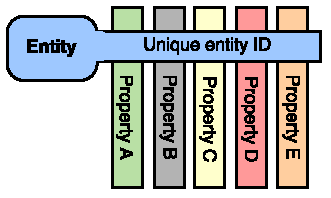
\includegraphics[width=0.5\linewidth]{img/tecnica/entity}
    % \caption{Example of entity with five properties. The entity id is used to access the information of all properties.}
    \caption[Exemplo de uma entidade]{Exemplo de uma entidade com cinco propriedades. O índice (ID) da entidade é utilizado para acessar as informações de todas as propriedades.}
    \label{fig:entity_example}
\end{figure}

\subsection{Sistema de Entidades}

O sistema de entidade é necessário para gerenciar o acessar as entidades e suas propriedades. Este sistema também é responsável por criar e destruir entidades, bem como gerenciar os vetores das propriedades ao alterar o número de entidades. Por exemplo, se uma entidade for criada ou destruída, o sistema da entidade deve assegurar de forma eficiente que todos os vetores permanecem contíguos na memória.

Além de gerenciar a criação e destruição de entidades, o sistema de entidade deve fornecer uma interface de acesso as entidades e suas propriedades com complexidade de tempo constante  ($\mathcal{O}(1)$). Para apresentar os algoritmos do sistema da entidade, vamos usar a notação descrita na Tabela~\ref{tab:notations}. Observe que $E_S$ e $P$ são vetores e, portanto, seus valores podem ser acessados através dos índices correspondentes. Por exemplo, $E_S(i)$ representa a entidade na i-ésima posição do vetor de entidades.

\begin{table}[!ht]
\centering
\caption{Notações utilizada no \textit{Entity-Component System} }
\label{tab:notations}
\resizebox{\linewidth}{!}{
\begin{tabular}{ c l }
\toprule[0.15em]
\textbf{Symbol}     & \textbf{Meaning}    \\ \midrule[0.1em]
$S$         & sistema de entidades $S$ \\
$e$         & entidade $e$ \\
$id_e$      & índice ($id$) da entidade $e$ \\
$E_S$       & vetor de entidades pertencente ao sistema de entidade $S$ \\
$E_S(i)$    & entidade armazenada na i-ésima posição do vetor $E$ \\
$\mathcal{P}_S$       & conjunto de propriedades associadas a um sistema de entidades $S$ \\
$P$         & vetor de propriedades $P$ \\
$P(j)$      & valor armazenado na j-ésima posição do vetor de propriedades $P$ \\ \bottomrule[0.15em]
% $C(e, e')$ & composition relationship between entities $e$ and $e'$ \\
% $A(e, e')$ & aggregation relationship between entities $e$ and $e'$ \\ \bottomrule[0.15em]
\end{tabular}
}
\end{table}

\simbolo{$S$}{sistema de entidades $S$}
\simbolo{$e$}{entidade $e$}
\simbolo{$id_e$}{índice ($id$) da entidade $e$}
\simbolo{$E_S$}{vetor de entidades pertencente ao sistema de entidade $S$}
\simbolo{$E_S(i)$}{entidade armazenada na i-ésima posição do vetor $E$}
\simbolo{$\mathcal{P}_S$}{conjunto de propriedades associadas a $S$}
\simbolo{$P$}{vetor de propriedades $P$}
\simbolo{$P(j)$}{valor armazenado na j-ésima posição de $P$}


O Algorítimo~\ref{alg:entityCreate} descreve como o sistema da entidade cria novas entidades. Quando uma nova entidade $ e $ é criada (linha 1), o sistema da entidade atribui a $ e $ um identificador $ id_e $ equivalente ao tamanho do vetor de entidades $ E_S $ (linha 2). Então a entidade $ e $ é inserida no final do vetor de entidades $ E_S $, chamando a função $ PUSH\_BACK $ (linha 3). Finalmente, para cada propriedade $P$ associada ao sistema da entidade $S$, um valor padrão é adicionado para a nova entidade $ e $ (linhas 4-6). Observe que o identificador de $ e $ ($ id_e $) é usado como um índice para acessar os vetores de propriedades.

\begin{algorithm}[ht]
%  \scriptsize
% \footnotesize
 \SetKwInOut{Input}{Input}\SetKwInOut{Output}{Output}
 \LinesNumbered
      \Input{Sistema de entidade $S$}
      \Output{Nova entidade $e$}
      $e \gets $ nova entidade\;
      $id_e \gets |E_S|$\;
      $PUSH\_BACK(E_S, e)$\;
      %$E(S) \gets E(S) \cup \{e\}$\;
      \ForEach{$P \in \mathcal{P}_S$}{
            $P(id_e) \gets$ valor padrão\;
      }
      \KwRet{$e$}\;
   \caption{ENTITY\_CREATE}
   \label{alg:entityCreate}
 \end{algorithm}

 O Algoritmo~\ref{alg:entityDestroy} apresenta as etapas de remoção de uma entidade. Dada uma entidade $ e $ para ser destruída, o sistema da entidade poderia simplesmente removê-lo do vetor de entidades. No entanto, remover um elemento do meio de um vetor contíguo tem uma complexidade de tempo de $\mathcal{O}(n)$, sendo $ n $ o número de entidades. Outra opção seria atribuir a entidade $ e $ como inválida, em vez de removê-la do vetor. No entanto, essa abordagem deixaria buracos no vetor de entidades, o que poderia degradar o desempenho do sistema da entidade.

  Em vez de remover a entidade $ e $ do vetor ou atribuí-la como inválida, o sistema de entidade substitui a entidade $e$ pela última entidade $e'$ do vetor de entidades (linhas 1-4). Em seguida, o último elemento deste vetor é removido ao chamar a função $ POP\_BACK $ (linha 5). Desta forma, o vetor de entidades permanece contíguo na memória e a operação de remoção é executada em~$\mathcal{O}(1)$. Depois de substituir $ e $ por $ e' $, o sistema de entidade faz o mesmo para os vetores de propriedades, substituindo os valores associados à entidade $ e $ por aqueles associados com a entidade $ e' $ (linhas 6-9). Por fim é retornado o sistema de entidades $S$ sem a entidade $e$.

 \begin{algorithm} [ht]
 %  \scriptsize
 % \footnotesize
  \SetKwInOut{Input}{Input}\SetKwInOut{Output}{Output}
  \LinesNumbered
       \Input{Sistema de entidade $S$, e entidade $e$ a ser removida}
       \Output{Sistema de entidade $S$ sem a entidade $e$}
         $n \gets |E_S|$\;
         $e' \gets E_S(n-1)$\;
         $E_S(id_e) \gets e'$\;
         $id_{e'} \gets id_e$\;
         $POP\_BACK(E_S)$\;
         \ForEach{$P \in \mathcal{P}_S$}{
             $P(id_e) \gets P(n-1)$\;
             $POP\_BACK(P)$\;
         }
         % $\mathcal{C} \gets \{C(e, e'') \mid e$ is composed by $e''\}$\;
         % \ForEach{$C(e, e'') \in \mathcal{C}$}{
         %     $DESTROY(C(e, e''))$\;
         %     $ENTITY\_DESTROY(S, e'')$\;
         % }
         % $\mathcal{A} \gets \{A(e, e'') \mid e$ is aggregated by $e''\}$\;
         % \ForEach{$A(e, e'') \in \mathcal{C}$}{
         %     $DESTROY(A(e, e''))$\;
         % }
         \KwRet{$S$}\;
    \caption{ENTITY\_DESTROY}
    \label{alg:entityDestroy}
  \end{algorithm}

  Em vez de usar relacionamentos hierárquicos (como \ac{ood}), o padrão de projeto \textit{Entity-Component System} representa relações entre as entidades por meio de composição e agregação. Uma composição representa uma relação de posse. Uma agregação, por sua vez, é simplesmente uma associação entre diferentes entidades, sem posse~\cite{gamma1995design}.
  % Figura \ref {} mostra exemplos de composição e agregações no contexto do design físico.
  Por exemplo, uma célula de circuito é composta por pinos, o que significa que, quando a célula é destruída, todos os seus pinos devem ser destruídos também. Por outro lado, a relação entre uma interconexão e seus pinos é simplesmente uma agregação. Como consequência, se uma interconexão é destruída, a relação também é destruída, mas todos os pinos permanecem no sistema da entidade.

  Esses relacionamentos podem ser adicionados à implementação do sistema de entidade (Algoritmos~\ref{alg:entityCreate} e~\ref{alg:entityDestroy}) como propriedades especiais. Desta forma, quando a propriedade é removida do vetor de propriedades (linha $ 8 $ do Algoritmo~\ref{alg:entityDestroy}), ele remove automaticamente o relacionamento. Além disso, se a propriedade é uma composição, serão removidas todas as entidades relacionadas.


% Com objetivo de mensurar quantitativamente o percentual de redução no número de cache misses e no tempo de execução, este trabalho irá analisar três tarefas de  Physical Design Automation.
% As subseções a seguir explanam como a organização dos dados
% -- ou --
% Este capítulo apresenta a proposta de organização dos dados para melhorar o desempenho de problemas de Physical Design Automation. Inicialmente, são discutidas as limitações do modelo de \ac{ood} e como o modelo de \ac{dod} pode sanar os mesmos. Em seguida, é discutido como o modelo \ac{dod} pode reduzir no número de cache misses. Por fim, são apresentados como podem ser aplicados os dois modelos (\ac{ood} e \ac{dod}) em três tarefas de Physical Design Automation.
%
% \section{Modelo de Programação Orientado a Objetos}
% \label{sec:modelo_orientado_objetos}
%
% Tipicamente, ferramentas de \ac{eda} são construídas utilizando o modelo de programação \ac{ood}.
% Este modelo decompõe o problema em objetos e mapeia estes objetos de mundo real para classes.
% Esses objetos são acessados através de uma interface bem definida e suas relações são representadas através da hierarquia, composição e agregação~\cite{booch2006object}.
% O modelo de programação \ac{ood} é popular porque geralmente há um mapeamento um-para-um entre os objetos do mundo real e seus objetos correspondentes no programa.
% Esta relação facilita a escrita e depuração do código.
%
%
% Para ilustrar os conceitos básicos aplicados no modelo de programação \ac{ood}, suponha que uma biblioteca de Physical Design precise ser desenvolvida.
% Esta biblioteca deverá solucionar uma ampla gama de problemas.
% Em seguida, assuma que um desenvolvedor de software deseja utilizar esta biblioteca para construir uma ferramenta que irá estimar o comprimento das interconexões (\textit{nets}) de um determinado circuito.
% A Figura~\ref{fig:circuito_exemplo} apresenta um exemplo de um circuito digital contendo quatro Nets e oito pinos.
%
%
% \begin{figure}[ht]
%     \centering
%     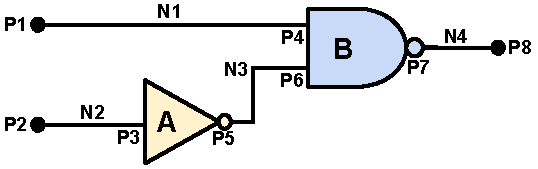
\includegraphics[width=0.7\linewidth]{img/tecnica/circuitExample}
%     % \caption{Combinational circuit portion with two logic gates (A and B), four nets (N1 to N4), and eight pins (P1 to P8).}
%     \caption[Fragmento de um circuito combinacional]{Fragmento de um circuito combinacional composto por duas portas lógicas (A e B), quatro nets (N1 a N4) e oito pinos (P1 a P8).}
%     \label{fig:circuito_exemplo}
% \end{figure}
%
% Um estimador de comprimento de interconexão deve ter acesso à informação de quais pinos pertencem a cada Net, bem como às posições dos pinos dentro do leiaute do circuito.
% A Figura~\ref{fig:classHierarchyOOD} ilustra uma possível decomposição para o problema de estimativa de comprimento de interconexão seguindo o modelo de programação \ac{ood}.
% Este diagrama é composto por dois módulos: \textit{Netlist} e \textit{Placemment}.
% O módulo \textit{Netlist} possui duas classes, \textit{Net} e \textit{Pin}, para descrever as interconexões do circuito e os pinos associados.
% Para a classe \textit{Pin}, este módulo caracteriza apenas o nome do pino e a rede a que ele pertence, sem qualquer informação de posicionamento.
% O módulo \textit{Placemment}, por sua vez, descreve as posições dos pinos.
% A seta entre as classes \textit{Pin} e \textit{Net} representam uma relação de agregação, o que significa que a interconeção possui uma referência aos seus pinos, enquanto um pino tem uma referência à sua interconeção proprietária.
% A seta entre as duas classes \textit{Pin} representa um relacionamento hierárquico, o que significa que a classe \textit{Pin} do módulo \textit{Placement} estende os atributos do pino do módulo \textit{Netlist}.
%
% \begin{figure}[ht]
%     \centering
%     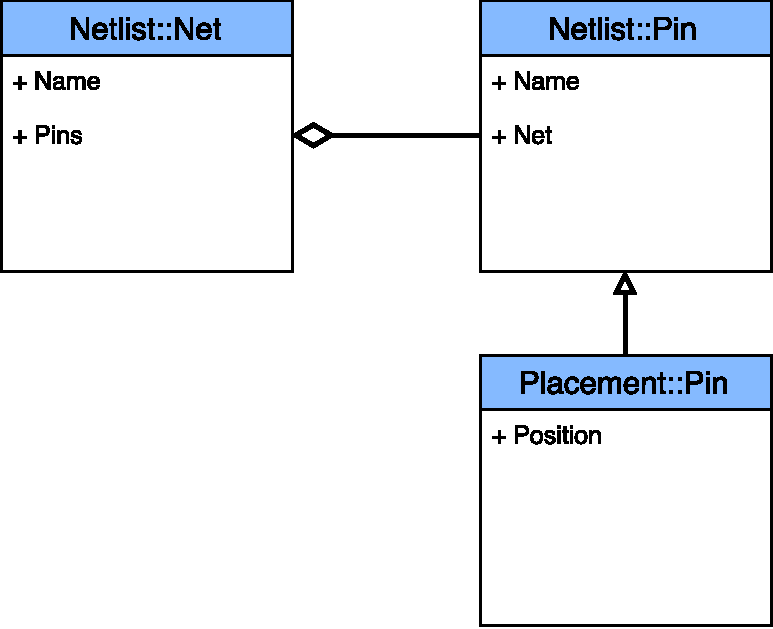
\includegraphics[width=0.5\linewidth]{img/tecnica/classHierarchyOOD}
%     % \caption{Class diagram to model wirelength estimation problem with \ac{ood} approach.}
%     \caption[Diagrama de classe com OOD]{Diagrama de classe para modelagem da estimativa do comprimento de uma intercenexão seguindo o modelo de programação \ac{ood}}
%     \label{fig:classHierarchyOOD}
% \end{figure}
%
% Embora possa ser fácil decompor um problema usando o modelo \ac{ood}, a implementação de um software, baseando-se apenas neste modelo de programação, pode levar a uma hierarquia de classes excessivamente complexa.
% Esta questão é particularmente crítica no desenvolvimento de uma biblioteca de software, pois é difícil prever, durante o design da biblioteca, como ela será realmente utilizada.
% Por exemplo, suponha que outro problema requer informações temporais sobre os pinos do circuito da Figura~\ref{fig:circuito_exemplo}.
% Seguindo o modelo de programação \ac{ood}, essas informações temporais podem ser adicionadas naturalmente criando um novo módulo chamado \textit{Timing} e uma nova classe \textit{Pin} (com atributos de temporização dos pinos) neste módulo.
% Por sua vez, esta nova classe deve também estender a classe \textit{Pin} do módulo \textit{Netlist}.
% Esta nova decomposição resulta na hierarquia de classes mostrada na Figura~\ref{fig:classHierarchyTimingOOD}.
%
% \begin{figure}[ht]
%     \centering
%     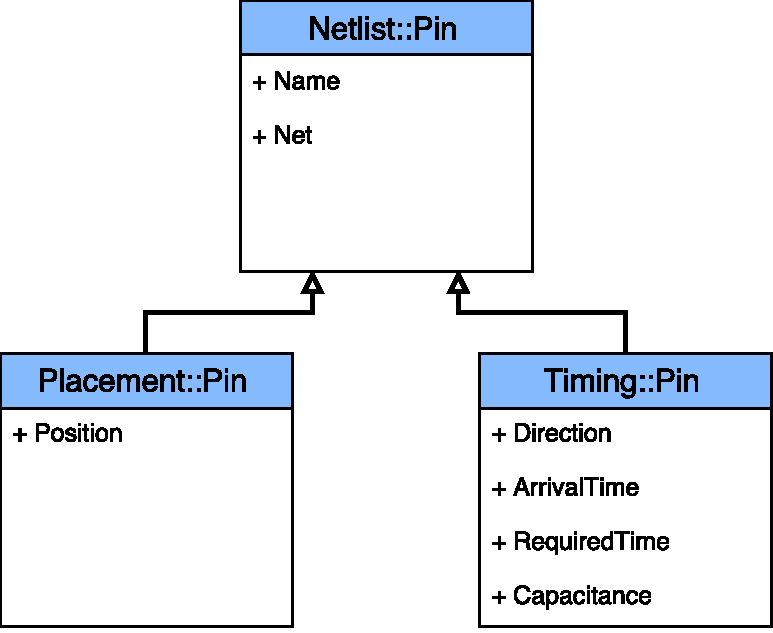
\includegraphics[width=0.5\linewidth]{img/tecnica/classHierarchyTimingOOD}
%     % \caption{Class diagram to model when pin timing information is added.}
%     \caption[Diagrama de classe de um pino]{Diagrama de classe de um pino com informações de posicionamento e temporais.}
%     \label{fig:classHierarchyTimingOOD}
% \end{figure}
%
%
% Agora, suponha que outro desenvolvedor queira usar nossa biblioteca de Physical Design para implementar um algoritmo de \ac{itdp}.
% Para fazer isso, este desenvolvedor irá precisar de uma nova classe \textit{Pin} com as informações de posicionamento e temporização.
% Em \ac{ood}, isso pode ser realizado através de herança múltipla, onde esta nova classe \textit{Pin} estende as classes \textit{Pin} de \textit{Placemment} e \textit{Timing}.
% No entanto, a herança múltipla não é suportada por todas as linguagens de programação, e mesmo quando suportada, não é recomendável porque pode levar a problemas de design~\cite{nystrom2014game}.
%
% Sem recorrer a herança múltipla, a solução consiste em criar uma nova classe \textit{Pin} que se estende do módulo \textit{Placement} ou \textit{Timing}, e repita o código da outra classe (que não foi estendida).
% Esta solução está apresentada na Figura~\ref{fig:classITDP}(a) e~\ref{fig:classITDP}(b).
% De qualquer forma, não existe uma maneira simples de reutilizar informações de posicionamento e tempo sem ocorrer replicação de código.
% A única opção restante é reunir todas as informações na classe \textit{Pin} do módulo \textit{Timing}, fazendo o mesmo estender o do módulo \textit{Placement}.
% Esta solução está ilustrada na Figura~\ref{fig:classITDP}(c).
% No entanto, nem sempre é necessário ter informações de posicionamento no módulo \textit{Timing}.
% Por exemplo, uma ferramenta analize de timing estática pode não precisar de informações de posicionamento durante etapas iniciais do projeto.
% Portanto, a adoção da última solução (Figura~\ref{fig:classITDP}(c)) levaria ao desperdício de memória, uma vez que informações desnecessárias seriam armazenadas.
%
% \begin{figure}[!ht]
%     \centering
%     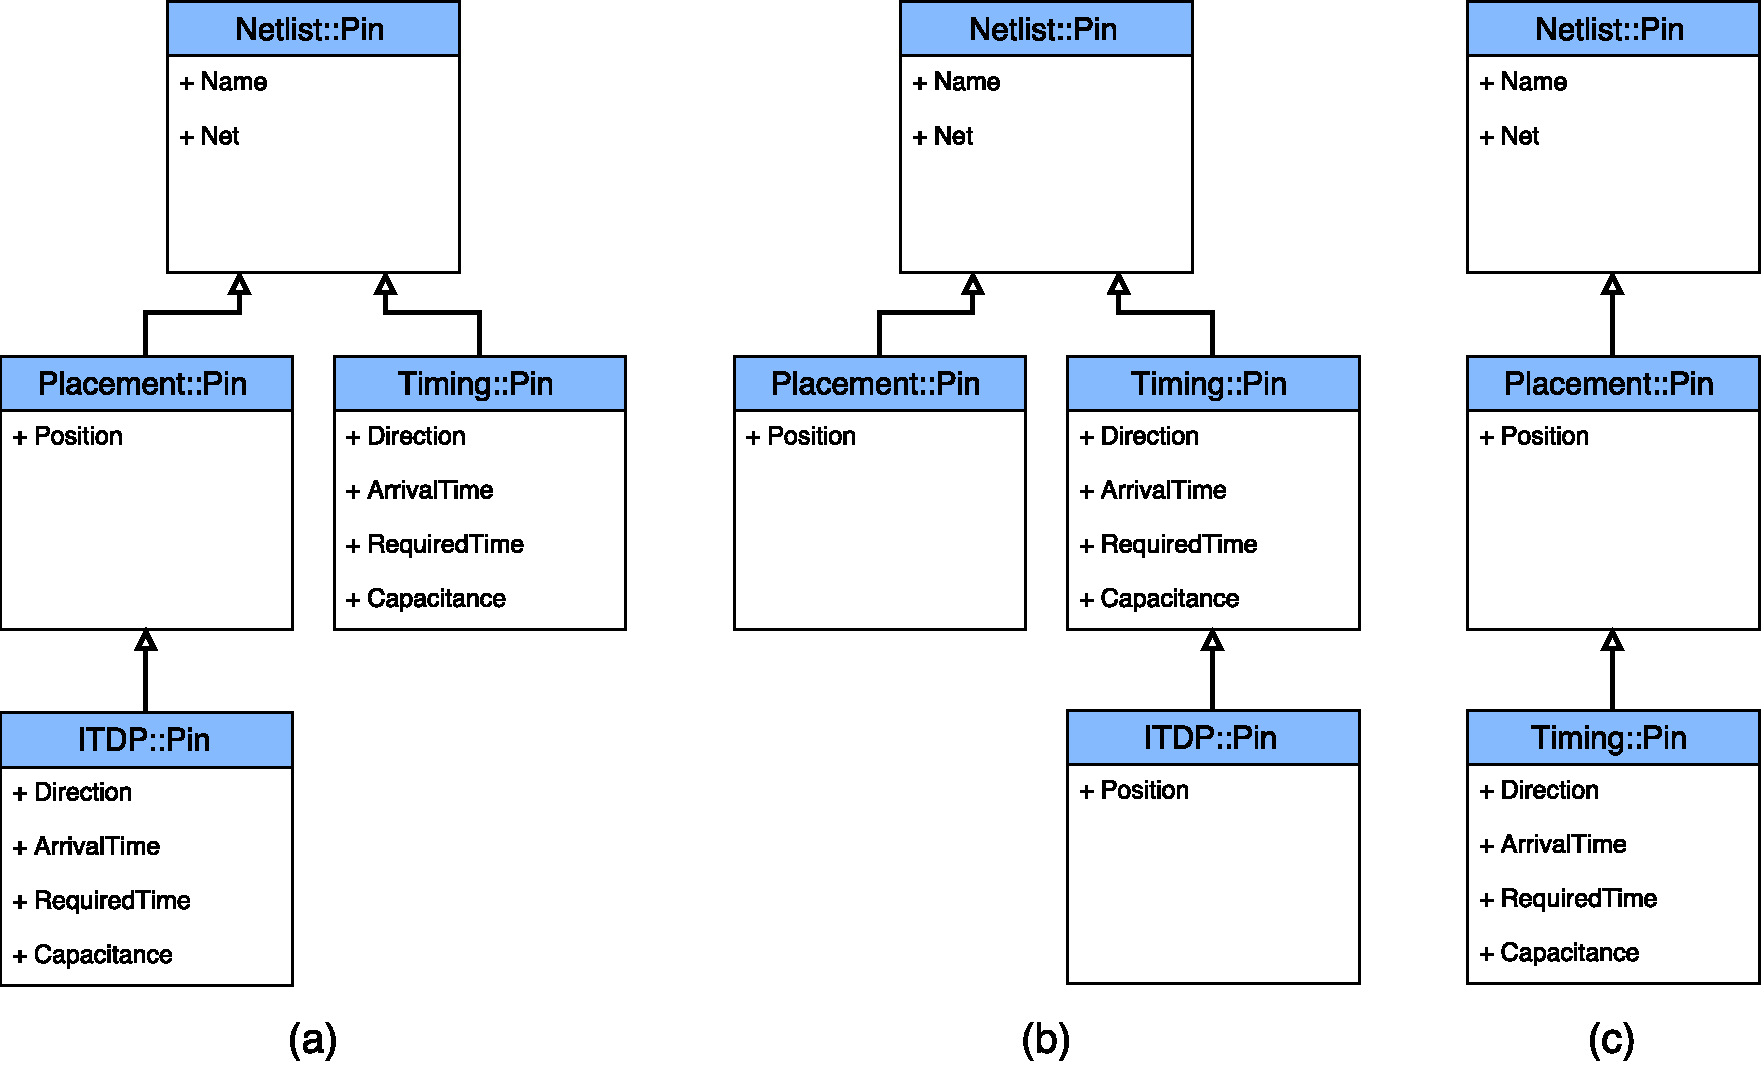
\includegraphics[width=\textwidth]{img/tecnica/ITDPsolutionOOD}
%     % \caption{Possible class hierarchy to support information of \textit{Timing} and \textit{Placement} for a timing-driven placement algorithm following \ac{ood} approach.}
%     \caption[Hierarquia de classes para suportar \textit{Timing} e \textit{Placement}]{Possível hierarquia de classes para suporte  informações de \textit{Timing} e \textit{Placement} para um algorítmo de \ac{itdp} seguindo o modelo de programação \ac{ood}.}
%     \label{fig:classITDP}
% \end{figure}




% \section{Modelo de Programação Orientado a Dados}
% \label{sec:modelo_orientado_dados}
%
% \section{Modelagem dos Dados para Physical Design}
% \label{sec:modelagem_physical_design}

% \subsection{Estudo de Caso A\@: Verificação dos Limites do Chip}
% \label{subsec:problema_A}

% \subsection{Estudo de Caso B\@: Estimativa de Interconexão}
% \label{subsec:problema_B}

% \subsection{Estudo de Caso C\@: Clusterização de Registradores}
% \label{subsec:problema_C}


% apresentar modelo de memoria
% apresentar como cache miss funciona
% apresentar ood
% apresentar limitação do ood
% apresentar dod
% apresentar entity system
% Discutir como o DOD reduz o numero de cache misses
% como aplicar o dod em problemas
%     Problema A - limites do chip
%         como seria modelado OOD
%         como seria modelado DOD
%     Problema B - interconexão
%         como seria modelado OOD
%         como seria modelado DOD
%     Problema C - cluster
%         como seria modelado OOD
%         como seria modelado DOD

% \chapter{Resultados Experimentais Preliminares}
\label{cap:resultados}

% Este capítulo apresenta os resultados experimentais obtidos por este trabalho. Inicialmente, ele descreve a infraestrutura experimental utilizada. Em seguida, analisa as três estratégias de legalização, no contexto de uma técnica de otimização incremental. Por fim, apresenta os resultados experimentais da avaliação da técnica proposta para legalização incremental.

\section{Infraestrutura experimental}
\label{sec:infraestrutura_experimental}

% Os experimentos realizados utilizaram o conjunto de benchmarks disponibilizados pela competição \textit{ICCAD 2015 CAD Contest (problem C: Incremental Timing-Driven Placement)} \cite{kim2015}, o qual inclui 8 circuitos que possuem entre 768k e 1,93M células, todos derivados de circuitos industriais. Para cada circuito, a infraestrutura da competição fornece um posicionamento inicial, o qual já está legalizado. Optou-se por utilizar tal infraestrutura pois a mesma disponibiliza circuitos com número de células compatível com circuitos contemporâneos. Além disso, tal infraestrutura é de acesso aberto, o que facilita a comparação experimental deste trabalho com futuros trabalhos que possivelmente serão realizados por terceiros.

% Todos os algoritmos apresentados neste capítulo foram implementados em C++. Para o desenvolvimento do protótipo com a técnica proposta, utilizou-se a implementação de R-tree disponível na biblioteca Boost \cite{boost}. Para fazer uso da R-tree é necessário definir dois de seus parâmetros: o grau da árvore e o algoritmo utilizado para a divisão de nodos durante a operação de inserção. Após alguns experimentos iniciais, não foi observada uma diferença significativa no tempo de execução das operações da R-tree ao variar o seu grau. Devido a isso, optou-se por utilizar uma árvore com grau 16. Por outro lado, o algoritmo de divisão de nodos utilizado tem impacto direto no tempo de execução da operação de inserção, assim como no tempo de execução das operações de busca subsequentes. Portanto, optou-se por utilizar o algoritmo denominado R*, que resulta em buscas espaciais mais rápidas, ao custo de um tempo de inserção um pouco maior.

% Todos os experimentos foram realizados em um computador Linux com quatro CPUs Intel\textsuperscript{\textregistered} Core\textsuperscript{\textregistered} i5-4460 @ 3,20 GHz e 32GB RAM. Os experimentos que avaliam o tempo de execução podem apresentar resultados diferentes em cada realização, devido a variações causadas pelo computador utilizado. Portanto, para aumentar a confiança estatística obtida pelos experimentos, os mesmos foram repetidos 10 vezes, o que resultou em 99\% de confiança estatística\footnote{A confiança estatística foi medida utilizando o teste t de Student para p=0,01.}. Como a confiança estatística obtida foi suficientemente alta, os experimentos não foram repetidos mais vezes.

\section{Comparação das estratégias de ...}

% \chapter{Cronograma}
\label{cap:cronograma}

Este capítulo apresenta as atividades já concluídas até o momento da escrita deste documento, assim como as atividades pendentes que serão realizadas após o exame de qualificação.

\section{Atividades concluídas}

% \begin{itemize}
%     \item \textbf{C1}: Implementar o algoritmo proposto de legalização incremental;
%     \item \textbf{C2}: Implementar os trabalhos relacionados em legalização incremental propostos em \citeonline{chow2014cell} e \citeonline{popovych2014density};
%     \item \textbf{C3}: Avaliar o algoritmo proposto comparando-o com os trabalhos relacionados da atividade \textbf{C2};
%     \item \textbf{C4}: Implementar o algoritmo Abacus descrito em \citeonline{spindler2008abacus} para avaliar as estratégias de legalização final e iterativa;
%     \item \textbf{C5}: Comparar quantitativamente as três estratégias de legalização: final, iterativa e incremental;
%     \item \textbf{C6}: Submeter artigos às conferências ISVLSI 2016 (Qualis B1) e SBCCI 2016 (Qualis B1).
% \end{itemize}

\section{Atividades pendentes}

% \begin{itemize}
%     \item \textbf{P1}: Realizar as sugestões de melhoria do trabalho propostas pela banca no exame de qualificação;
%     \item \textbf{P2}: Apresentar o artigo no ISVLSI 2016;
%     \item \textbf{P3}: Apresentar o artigo no SBCCI 2016;
%     \item \textbf{P4}: Escrever a dissertação de mestrado;
%     \item \textbf{P5}: Preparar a apresentação e defender este trabalho de mestrado;
%     \item \textbf{P6}: Realizar as correções sugeridas pela banca durante a defesa;
%     \item \textbf{P7}: Entregar a versão final da dissertação de mestrado na Biblioteca Central da Universidade Federal de Santa Catarina.
% \end{itemize}

\section{Cronograma}

% A Figura \ref{tab:cronograma} apresenta o cronograma o previsto para realização deste trabalho de mestrado. Os meses de Junho a Agosto serão dedicados às correções sugeridas pela banca no exame de qualificação, assim como à apresentação do artigo aceito no ISVLSI 2016. Finalizando as correções, a dissertação será escrita a partir de Setembro, tendo sua finalização prevista em Novembro, quando inicará a preparação para a defesa, prevista para Dezembro. Por fim, os meses de Janeiro e Fevereiro são reservados para realizar as correções sugeridas pela banca na defesa e entrega do artigo na Biblioteca Central da Universidade Federal de Santa Catarina. Desta forma, a finalização deste trabalho de mestrado está dentro do prazo de 24 meses previsto pelo programa de Pós-Graduação em Ciência da Computação da Universidade Federal de Santa Catarina.

% \begin{table}[ht]
% \centering
% \resizebox{\textwidth}{!}{
% \begin{tabular}{@{}cccccccccc@{}}
% \toprule
%                                   & \textbf{Junho}         & \textbf{Julho}         & \textbf{Agosto}        & \textbf{Setembro}      & \textbf{Outubro}       & \textbf{Novembro}      & \textbf{Dezembro}      & \textbf{Janeiro}       & \textbf{Fevereiro}     \\ \midrule
% \multicolumn{1}{|c|}{\textbf{P1}} & \cellcolor[HTML]{FFFE65} & \cellcolor[HTML]{FFFE65}                      & \multicolumn{1}{c|}{\cellcolor[HTML]{FFFE65}} & \multicolumn{1}{c|}{}                         & \multicolumn{1}{c|}{}    & \multicolumn{1}{c|}{}                         & \multicolumn{1}{c|}{}                         & \multicolumn{1}{c|}{}    & \multicolumn{1}{c|}{}                         \\ \midrule
% \multicolumn{1}{|c|}{\textbf{P2}} & \multicolumn{1}{c|}{}    & \multicolumn{1}{c|}{\cellcolor[HTML]{FFFE65}} & \multicolumn{1}{c|}{}                         & \multicolumn{1}{c|}{}                         & \multicolumn{1}{c|}{}    & \multicolumn{1}{c|}{}                         & \multicolumn{1}{c|}{}                         & \multicolumn{1}{c|}{}    & \multicolumn{1}{c|}{}                         \\ \midrule
% \multicolumn{1}{|c|}{\textbf{P3}} & \multicolumn{1}{c|}{}    & \multicolumn{1}{c|}{}                         & \multicolumn{1}{c|}{}                         & \multicolumn{1}{c|}{\cellcolor[HTML]{FFFE65}} & \multicolumn{1}{c|}{}    & \multicolumn{1}{c|}{}                         & \multicolumn{1}{c|}{}                         & \multicolumn{1}{c|}{}    & \multicolumn{1}{c|}{}                         \\ \midrule
% \multicolumn{1}{|c|}{\textbf{P4}} & \multicolumn{1}{c|}{}    & \multicolumn{1}{c|}{}                         & \multicolumn{1}{c|}{}                         & \cellcolor[HTML]{FFFE65}                      & \cellcolor[HTML]{FFFE65} & \multicolumn{1}{c|}{\cellcolor[HTML]{FFFE65}} & \multicolumn{1}{c|}{}                         & \multicolumn{1}{c|}{}    & \multicolumn{1}{c|}{}                         \\ \midrule
% \multicolumn{1}{|c|}{\textbf{P5}} & \multicolumn{1}{c|}{}    & \multicolumn{1}{c|}{}                         & \multicolumn{1}{c|}{}                         & \multicolumn{1}{c|}{}                         & \multicolumn{1}{c|}{}    & \cellcolor[HTML]{FFFE65}                      & \multicolumn{1}{c|}{\cellcolor[HTML]{FFFE65}} & \multicolumn{1}{c|}{}    & \multicolumn{1}{c|}{}                         \\ \midrule
% \multicolumn{1}{|c|}{\textbf{P6}} & \multicolumn{1}{c|}{}    & \multicolumn{1}{c|}{}                         & \multicolumn{1}{c|}{}                         & \multicolumn{1}{c|}{}                         & \multicolumn{1}{c|}{}    & \multicolumn{1}{c|}{}                         & \multicolumn{1}{c|}{}                         & \cellcolor[HTML]{FFFE65} & \multicolumn{1}{c|}{\cellcolor[HTML]{FFFE65}} \\ \midrule
% \multicolumn{1}{|c|}{\textbf{P7}} & \multicolumn{1}{c|}{}    & \multicolumn{1}{c|}{}                         & \multicolumn{1}{c|}{}                         & \multicolumn{1}{c|}{}                         & \multicolumn{1}{c|}{}    & \multicolumn{1}{c|}{}                         & \multicolumn{1}{c|}{}                         & \multicolumn{1}{c|}{}    & \multicolumn{1}{c|}{\cellcolor[HTML]{FFFE65}} \\ \bottomrule
% \end{tabular}
% }
% \caption{Cronograma previsto para realização do trabalho de mestrado}
% \label{tab:cronograma}
% \end{table}
% \input{capitulos/conclusoes}

\bibliographystyle{ufsc-alf}
\bibliography{references}

%--------------------------------------------------------
% Elementos pós-textuais
\apendice
\chapter{Lista de Publicações}
\label{ap:producoes}
\section{Artigos publicados diretamente relacionados ao tema de mestrado}

A avaliação quantitativa da melhoria na organização dos dados, resultou em duas publicações diretamente relacionadas ao tema deste trabalho de mestrado. Os detalhes destas publicações estão listados nesta Seção.

\subsection{\textit{Proceedings of the 2017 ACM on International Symposium on Physical Design.}, 2017}

A Avaliação do impacto causado pelo número de caches misses em duas tarefas da síntese física de circuitos integrados, resultou na publicação de um atrigo completo no ISPD2017 --- International Symposium on Physical Design.

\begin{itemize}
\item \textbf{Qualis CC:} B1
\item \textbf{Título:} \textit{How Game Engines Can Inspire EDA Tools Development: A use case for an open-source physical design library}
\item \textbf{Autores:}  \textbf{Tiago Augusto Fontana}; Renan Netto; Vinicius Livramento; Chrystian Guth; Sheiny Almeida; Laércio Pilla; José Luís Güntzel
\item \textbf{DOI:} http://dx.doi.org/10.1145/3036669.3038248
\item \textbf{\textit{Abstract:}} \emph{Similarly to game engines, physical design tools must handle huge amounts of data. Although the game industry has been employing modern software development concepts such as data-oriented design, most physical design tools still relies on object-oriented design. Differently from object-oriented design, data-oriented design focuses on how data is organized in memory and can be used to solve typical object-oriented design problems. However, its adoption is not trivial because most software developers are used to think about objects' relationships rather than data organization. The entity-component design pattern can be used as an efficient alternative. It consists in decomposing a problem into a set of entities and their components (properties). This paper discusses the main data-oriented design concepts, how they improve software quality and how they can be used in the context of physical design problems. In order to evaluate this programming model, we implemented an entity-component system using the open-source library Ophidian. Experimental results for two physical design tasks show that data-oriented design is much faster than object-oriented design for problems with good data locality, while been only sightly slower for other kinds of problems.}
\end{itemize}


\subsection{\textit{Proceedings of the 30th Symposium on Integrated Circuits and Systems Design}, 2017}

A avaliação do impacto na exploração da localidade da cache utilizando Data-Oriented Design (DOD) no contexto de clusterização de registradores gerou o trabalho denominado "Exploiting Cache Locality to Speedup Register Clustering", o qual foi apresentado oralmente e publicado nos anais do SBCCI2017 --- 30th Symposium on Integrated Circuits and Systems Design.

\begin{itemize}
\item \textbf{Qualis CC:} B2
\item \textbf{Título:} \textit{Exploiting Cache Locality to Speedup Register Clustering}
\item \textbf{Autores:}  \textbf{Tiago Augusto Fontana}; Sheiny Almeida; Renan Netto; Vinicius Livramento; Chrystian Guth;  Laércio Pilla; José Luís Güntzel
\item \textbf{DOI:} http://dx.doi.org/10.1145/3109984.3110005
\item \textbf{\textit{Abstract:}} \emph{Physical design tools must handle huge amounts of data in order to solve problems for circuits with millions of cells. Traditionally, Electronic Design Automation tools are implemented using Object-Oriented Design. However, using this paradigm may lead to overly complex objects that result in waste of cache memory space. This memory wasting harms cache locality exploration and, consequently, degrades software runtime. This work proposes applying Data-Oriented Design on the register clustering problem. Differently from the traditional Object-Oriented design, the Data-Oriented Design programming model focus on how the data is organized in the memory. As consequence, this programming model may better explore cache spatial locality. In order to evaluate the impact of using the Data-Oriented Design programming model for register clustering, we implemented two software prototypes (a sequential and a parallel implementation) of the K-means clustering algorithm for each programming model. Experimental results showed that the sequential Data-Oriented Design implementation is on average $7.5\%$ faster when compared to the Object-Oriented Design implementation, while its parallel version is $15\%$ faster when compared to the Object-Oriented one.}
\end{itemize}


\end{document}
%%%%%%%%%%%%%%%%%%%%%%%%%%%%%%%%%%%%%%%%%%%%%%%%%%%%%%%%%%%%%%%%%%%%%%%
% Fim do documento
%%%%%%%%%%%%%%%%%%%%%%%%%%%%%%%%%%%%%%%%%%%%%%%%%%%%%%%%%%%%%%%%%%%%%%%
